% Pallu
% School of Engineering
% Machine Learning Assignment
% Northeastern University
% Boston, MA 02115

% Do not manipulate any of the settings
\documentclass[11pt]{article}
\renewcommand{\baselinestretch}{1.0} 
\usepackage{epsfig}
\usepackage{units}
\usepackage{amssymb}
\usepackage{amsmath}
\usepackage{fancyhdr}
\usepackage{amsmath}
\usepackage{enumitem}
\usepackage{graphicx}
\usepackage{subcaption}
\usepackage{listings}
\usepackage{floatrow}
\usepackage{csquotes}
\usepackage[utf8]{inputenc}
\usepackage{geometry}
\usepackage{authblk}
\usepackage{blindtext}
\usepackage{titlesec}
\usepackage{subfig}
\usepackage{lipsum}
\usepackage{wrapfig}
\geometry{margin=1in}
\graphicspath{ {} }
\DeclareMathOperator*{\argmax}{argmax}


\setlength{\oddsidemargin}{0 in}
\setlength{\evensidemargin}{0 in}
\setlength{\topmargin}{-0.6 in}
\setlength{\textwidth}{6.5 in}
\setlength{\textheight}{8.5 in}
\setlength{\headsep}{0.75 in}
\setlength{\parindent}{0 in}
\setlength{\parskip}{0.1 in}

\begin{document}
\title{\textbf{INFO6205 Project: Viral Diseases Simulator}
}
\author{Manik Kumar, Pallak Singh, Yatish Pitta}
\affil{\textit {\{kumar.man, singh.pal, pitta.y\}@northeastern.edu}}
\maketitle
\begin{abstract}
Infectious diseases continue to remain one of the major causes of morbidity in humans and animals alike all across the world. The frequency of outbreaks that have been reported over the past few decades has increased by a concerning amount. More recently, the newly identified SARS-Cov-2 has led to a large number of deaths along with over 50 million cases worldwide. As of December 8 2020, there haven't been any publicly administered vaccines released to control the impact of COVID-19 thereby, there has been extensive research not just in therapy for the infected but for controlling the spread of the disease itself. This requires cooperation between the government, the scientists and the general public in order to have an effective response. With the current pandemic, one can see that there has been resistance within the general public when it comes to following social distancing advisories and mask mandates which can be attributed to the lack of awareness when it comes to how viruses work and how they can be controlled. This project worked towards building an application capable of simulating a typical spread of viral diseases and how the spread and the impact of the disease varies depending on factors like K and R values, social distancing, mortality rates, mask mandates and even the specific effectiveness of a particular of mask. We also provided a helpful UI for better accessibility and information regarding each of the factors taken into consideration.

\end{abstract}
\pagestyle{fancy}
\renewcommand{\headrulewidth}{0pt}
\renewcommand{\footrulewidth}{0pt}
\fancyhf{}
\rfoot{\thepage}

%%
%% Objectives and Significance
%%
\section{Introduction}
With the spread of the virus SARS-Cov-2, which has now been named COVID-19 by World Health Organization, the world has found itself struggling on all fronts. From the dwindling economy to the overwhelmed healthcare capacity, this pandemic has been unpredictable and devastating. With the cases still surging and showing different behaviors in different areas, researchers are turning to mathematical models to predict how the disease is spreading. These models take into account different factors related to the virus along with specific population factors and simulate how the virus will behave. Simulation models can be useful not only to researchers, but also to the general public in order to understand a virus without the scientific jargon and visualize the impact of the measures being taken to control its spread. This encouraged us to build a tool that is accessible to a non-scientist and allows them to tweak different factors to see how it impacts the spread and effects of a virus. 

\begin{figure}[H]
\caption{Simulation on the Viral Diseases Simulator}\label{wrap-fig:1}
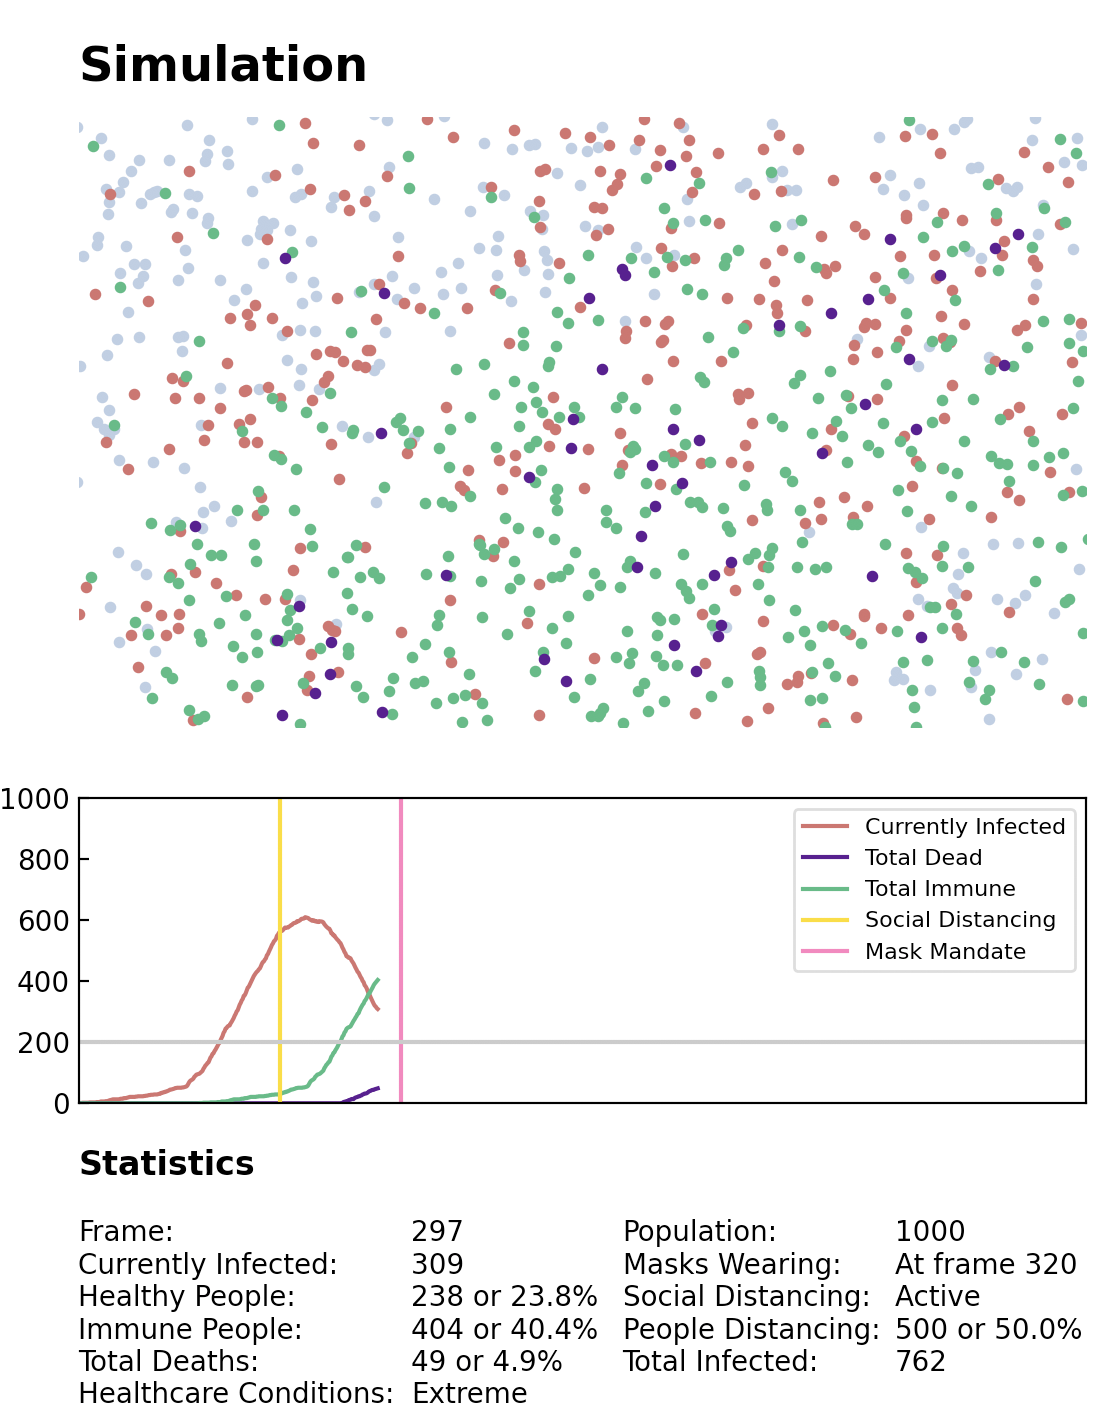
\includegraphics[width=8cm]{figures/intro-simulation.png}
\end{figure} 

Our application is a Viral Disease Simulator capable of visualizing  the spread of a viral disease, providing real-time graphs and statistics to better understand the simulation. As shown in Figure 1, one can easily visualize how social distancing, mask mandates, hospital capacity affect the statistics. 


We also provide a helpful UI which allows the user to modify configuration in order to simulate different scenarios. Our application comes with data loaded for the Influenza and COVID-19 disease. Users can customize virus related configurations to create their own scenarios.

\section{Aim}
The aim of this project is to model and simulate the spread of viral diseases such as COVID-19 and Influenza, and understand how factors like the K value, R value, population density, infection range, mortality rate and different intervention policies like social distancing, mask mandates, and travel restrictions impact the outcome of the viral outbreak. Our goal is also to provide a helpful GUI to interact with the application easily and provide an option to the users to tweak various factors and simulate how the virus behaves if that factor is changed. For complete understanding of the model, our aim is to be as comprehensible as possible through the means of charts and graphs.

\section{Project Details}

\textbf{Viral Diseases Simulator} is a stochastic simulation model that can project the spread of different viral diseases. The model works by taking into account the R and K factors of the disease, the mortality rate, recovery time and projecting the number of infections and state of the outbreak based on the healthcare capacity, intervention, and protection policies. 

The program is written in Python, with the help of the numpy library to aid in the mathematical modelling of the diseases. The computer graphical simulation is done using the Matplotlib library and the graphical user interface is written in Python, with the help of the Tkinter package and ttk module for styling. 

Visualization style used in this project was inspired by Paul Val Gent's Covid visualization\cite{sim_ref}. And certain elements in designing the algorithm were inspired by Grant Sanderson's YouTube videos discussing the current pandemic\cite{yt1}\cite{yt2}.

Details for the implementation and the final deliverable can be found in section 4 and section 6. The executable binaries of the application is available for macOS, Windows and Linux on the project repository on GitHub. 

\subsection{Features}

The program provides the functionality to simulate any viral disease by allowing the user to configure different parameters specific to the disease. All parameters available to the user and their respective functions are provided in section 6. All details regarding the algorithm can be found in section 5.

The application comes in built with configuration data for two diseases – 
\begin{enumerate}
    \item \textbf{COVID-19} gathered from \cite{cov_ref},\cite{k_val}
    \item \textbf{Influenza} gathered from \cite{influ_ref},\cite{k_val}
\end{enumerate}

The simulation can be observed in two modes:
\begin{enumerate}
    \item \textbf{Render Mode} Renders the simulation into a .mp4 video file on the disk. User can select the render mode from the radio buttons present on the right of the UI screen. 
    \item \textbf{Live Simulation Mode} Displays the simulation live on a matplotlib window. 
\end{enumerate}

User also has the option to run the application in two modes:
\begin{enumerate}
    \item \textbf{GUI (Graphical User Interface) mode:} This mode allows the user to configure different parameters of the simulation model through an intuitive UI and observe the simulation as they make the changes. The UI can be seen in \ref{ui-vis}.
    
    \begin{figure}[H]
    \centering
    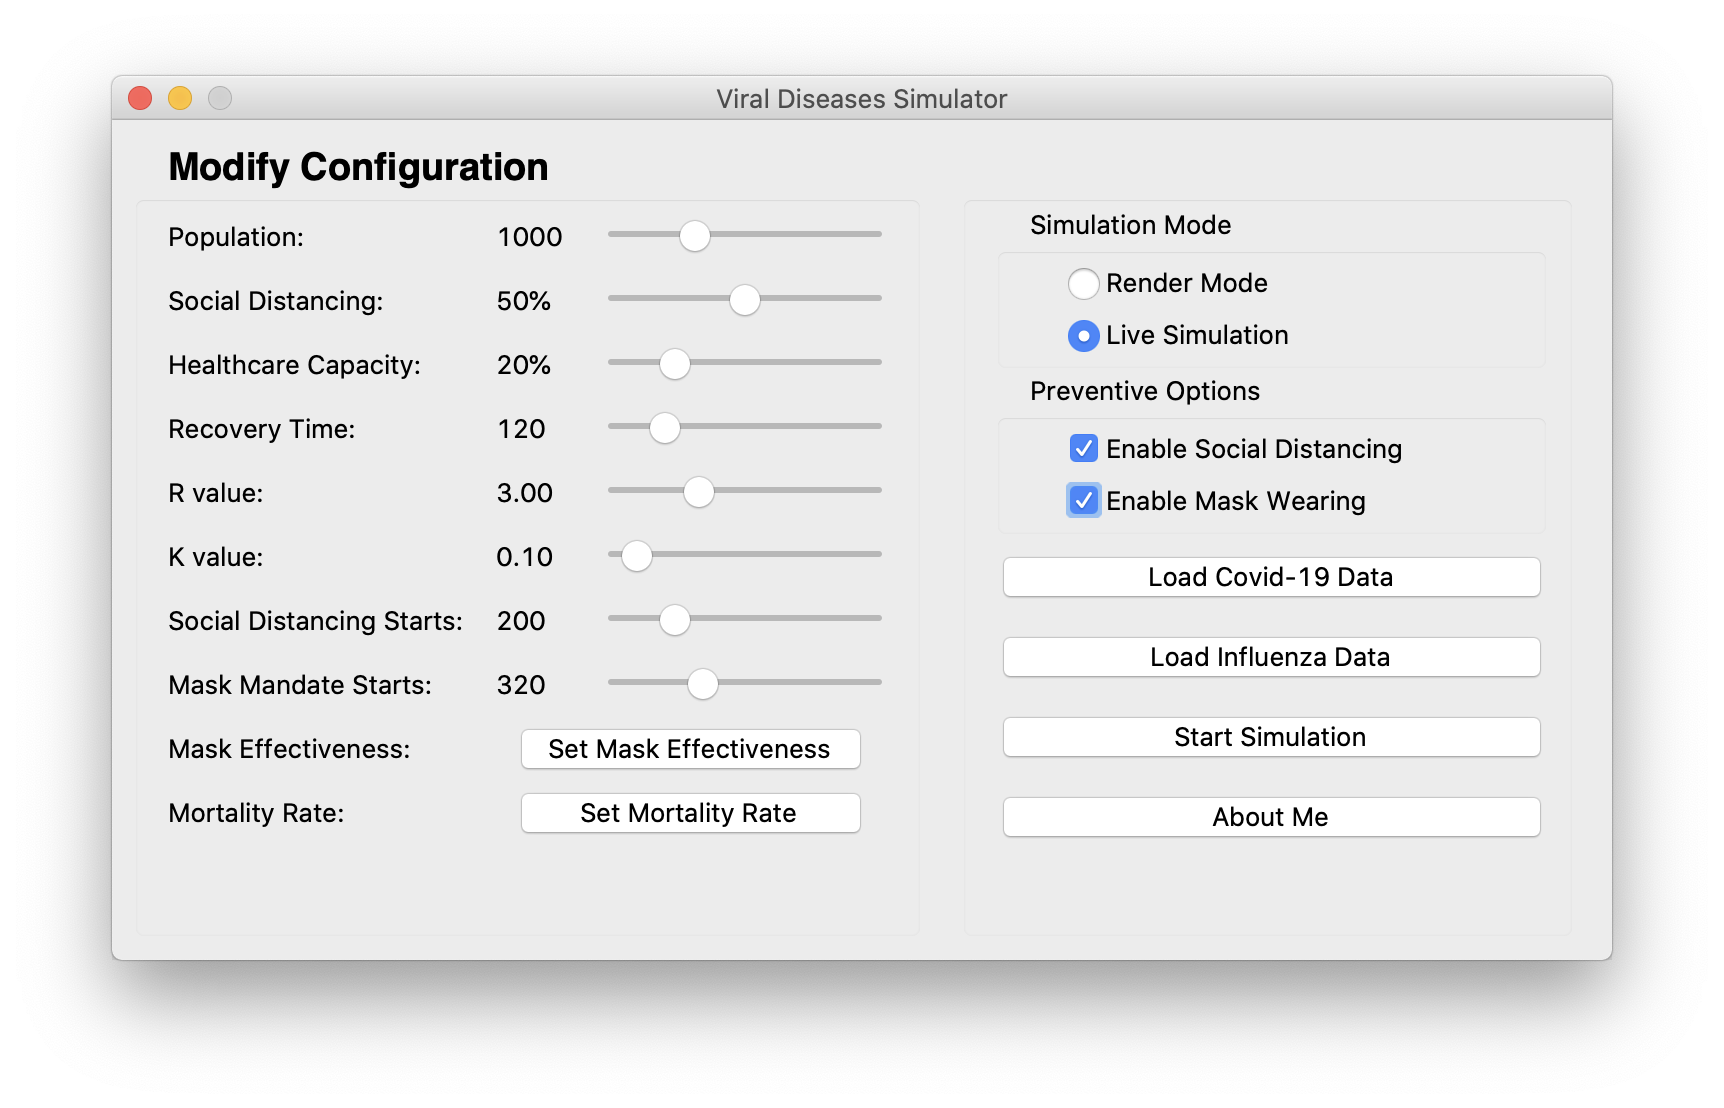
\includegraphics[width=14cm]{figures/ui-vis.png}
    \caption{GUI screen user is welcomed with}
    \label{ui-vis}
\end{figure}

\item \textbf{CLI mode:} This mode allows the user to run the simulation without the need to interact with the GUI. The simulation can be configured through the config/config.ini file. This will default to covid.stats portion of the config when it comes to variables that define the characteristics of a virus(stuff like K or R value). Change the values in the covid.stats to change virus characteristics. The user can can run the application in the CLI mode by entering the following command on their terminal:
\begin{lstlisting}
python main.py --disable-UI
\end{lstlisting}
\end{enumerate}
\subsection{Structure of the Application}
The core algorithm is located in the /src folder and contains all the modules necessary for the simulation. 


The /gui folder contains the code for the graphical user interface built using Tkinter.


The /test folder contains all the unit tests for the model.


The following are the core modules of the model:
\begin{enumerate}
    \item \textbf{config\textunderscore util.py:} Contains the ConfigUtil class, which has the functionality to parse configuration files and return configuration values.
    \item \textbf{population.py:}  Contains the Population class, which holds the main data container containing the information about each person. It also has methods to initialize the data container, and getters and setters for every data type. 
    \item \textbf{population\textunderscore util.py:}  Contains the PopulationUtil class, which is used to instantiate the Population class by passing in the appropriate configuration values from the configuration file. It also contains the move method, which is called at every frame interval and does the heavy lifting of calling the update methods to update the positions of each individual and calling the infect method.
    \item \textbf{virus\textunderscore util.py:} Contains the Virus class, which contains the main utility methods to infect individuals based on different factors and update the state of each individual.
    \item \textbf{movements.py:} Contains the Movement class, which contains utility functions to update the position of individuals on the X-Y plane.
    \item \textbf{visualization.py:} Contains the Visualization class, which makes use of the matplotlib library to plot the population and simulate the model.
\end{enumerate}

The UML diagram representing the core modules and how our application is designed to include those modules is provided in Figure \ref{uml-diag}.
 \begin{figure}[H]
    \centering
    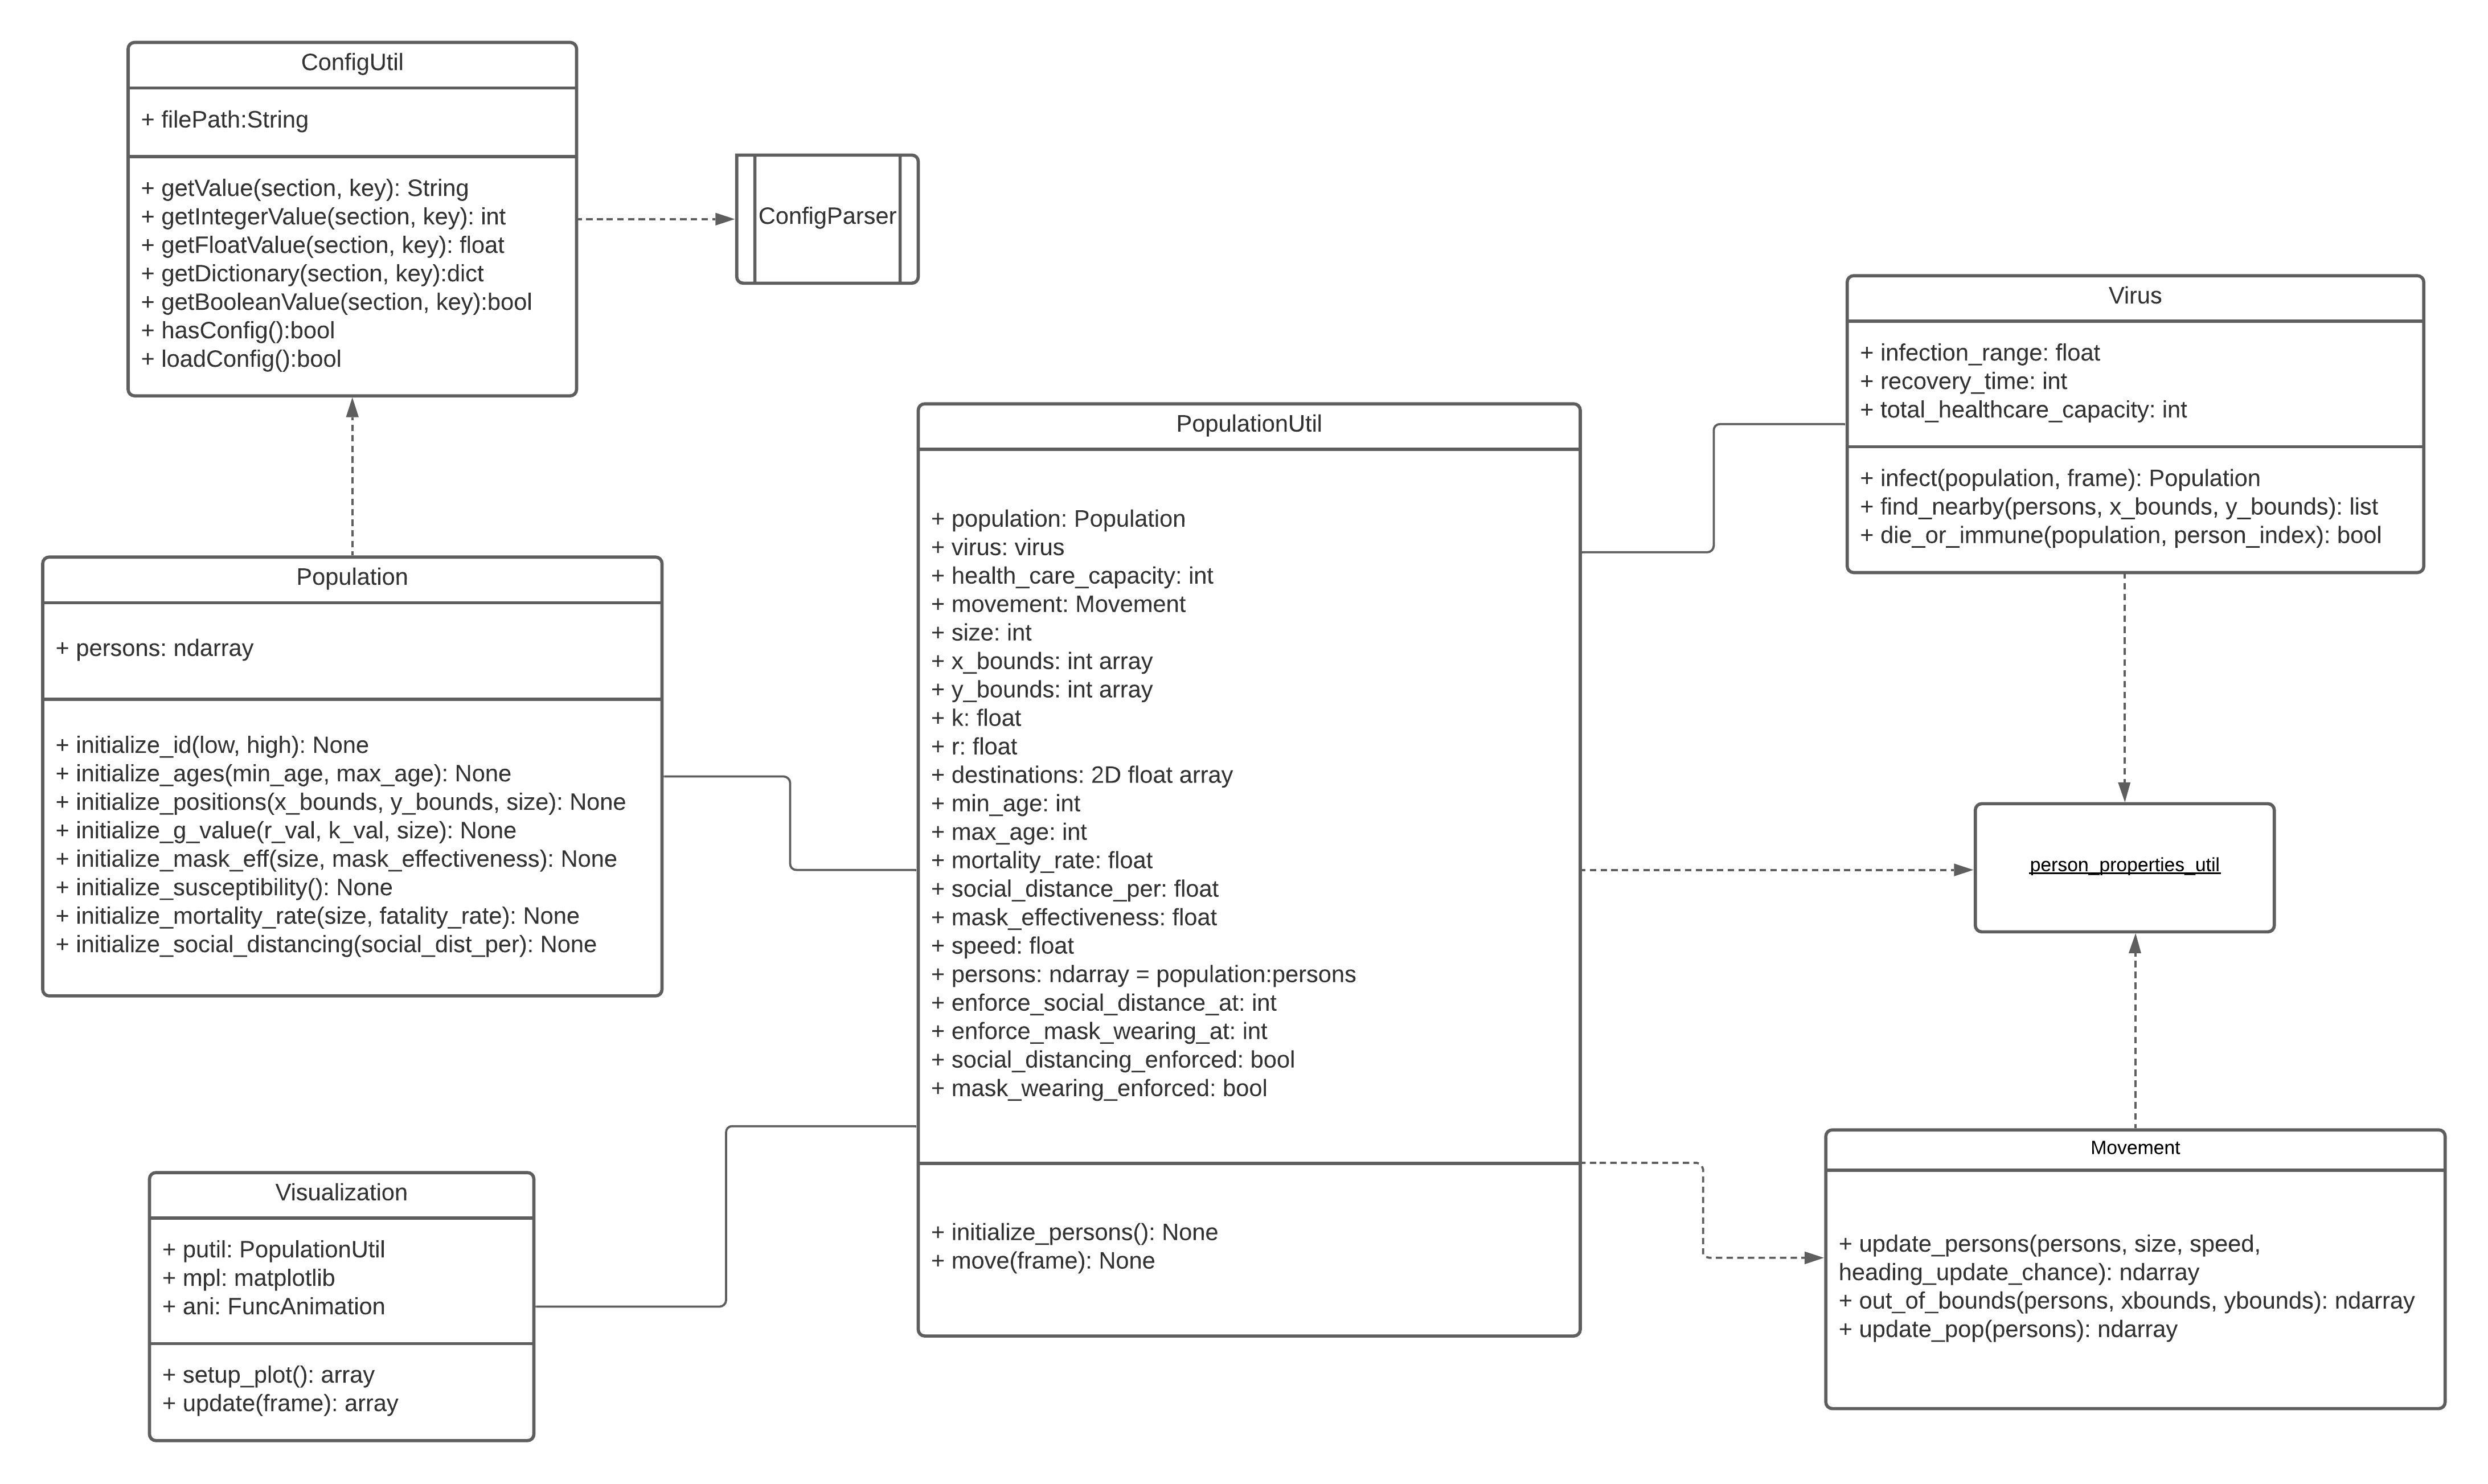
\includegraphics[width=18cm]{figures/umlDiag.JPG}
    \caption{UML diagram representing the core modules of the model}
    \label{uml-diag}
\end{figure}

\section{Implementation}
\subsection{Data Used for Model}
% Notes about how our algorithm works:

% Starting point: A matrix with 17 columns to store the individual variables for each individual, rows = number of people

% Individual Variables : 
% 1. Individual ID
% 2. age
% 3. Starting Position X
% 4. Starting Position Y
% 5. Where this guy is heading X
% 6. Where this guy is heading Y
% 7. wander range x
% 8. wander range y
% 9. Current state - ill, dead, or immune
% 10. g value i.e. individual R value, or how many people this guy will infect
% 11. mast effectiveness 
% 12. social distancing
% 13. overall susceptibility
% 14. Mortality
% 15. speed
% 16. Infected Time
% 17. was he infected

To create a sufficiently competent model, we start with loading in various statistics about the virus we're trying to model. Using those values and other user provided data, a set of random individuals are initialized which will contain various different variables using which the model algorithm will work.

The following virus statistics are being used.
\begin{enumerate}
    \item \textbf{R Value:} R value or the reproduction number is defined as the average number of individuals an infected person will infect over the course of the spread \cite{r_val}.
    \item \textbf{K Value:} K value or the dispersion value is defined as the variance in the number of individuals an infected person will infect \cite{k_val}.
    \item \textbf{Infection Range:} The physical distance under which it's plausible for an infected individual to spread the virus to someone else.
    \item \textbf{Mask Effectiveness:} This defines how effective masks are in protecting a healthy individual when they come within the infection range of an infected person. Mask effectiveness are defined for the following different masks.
    \begin{enumerate}
        \item Cloth Masks
        \item Surgical Masks
        \item N95 Masks
    \end{enumerate}
    \item \textbf{Mortality Rate:} This defines mortality rate of the virus for the following age ranges.
    \begin{enumerate}
        \item 0 to 19 years old.
        \item 29 to 49 years old.
        \item 50 to 69 years old.
        \item 70 years old and above.
    \end{enumerate}
    \item \textbf{Recovery Time:} This defines how long on an average it takes for someone to recover from the virus.
\end{enumerate}

The user provides following data-points using which different kinds of simulations can be visualized.
\begin{enumerate}
    \item The size of the population.
    \item What the healthcare capacity is.
    \item If there would be any social distancing measures
    \item How many individuals will respect the social distancing measures.
    \item When would the social distancing measures start.
    \item If there would be mask mandates.
    \item When would the mask mandates start
\end{enumerate}

To create a model that was sufficiently fast enough to update in real time and produce a simulation we decided to use matrices to store individual variables. The matrix storing all the data has 17 data columns,
\begin{enumerate}
    \item \textbf{ID:} Every individual is assigned a unique ID.
    \item \textbf{Age:} Stores the Age of the individual.
    \item \textbf{Starting Position X-axis:} X-axis of the position this individual will start from.
    \item \textbf{Starting Position Y-axis:} Y-axis of the position this individual will start from.
    \item \textbf{X-axis Heading:} X-axis of the direction this individual will be heading towards.
    \item \textbf{Y-axis Heading:} Y-axis of the direction this individual will be heading towards.
    \item \textbf{Wander Range X:} X-axis range of where an individual can wander in.
    \item \textbf{Wander Range Y:} Y-axis range of where an individual can wander in.
    \item \textbf{Speed:} Speed of movement of an individual.
    \item \textbf{Current State:} Current health status of the individual, e.g: Healthy, Immune, or Deceased.
    \item \textbf{Individual Infection Value:} Number of individuals this individual has the potential to infect if infected. This value is determined through a normal distribution taking in the R and K values of the virus.
    \item \textbf{Mask Effectiveness:} If this individual would wear a mask, if yes what kind of mask(e.g: cloth mask, N95, or surgical mask) and how effectively would it protect against the virus.
    \item \textbf{Social Distancing:} If this individual will participate in social distancing or not.
    \item \textbf{Susceptibility:} How susceptible is this individual for catching the virus, this field depends upon the infection range of the virus, what kind of mask the individual is wearing and if they're social distancing.
    \item \textbf{Mortality:} Percentage that determines an individuals mortality chance. This value depends upon on the individual's age, how deadly the virus is, and if healthcare capacities are full. If healthcare capacity conditions are extreme, mortality rates rise.
    \item \textbf{Infected At:} Stores when this individual was infected at for algorithmic purposes.
    \item \textbf{Hospitalization Status:} Stores whether or not this person was hospitalized.
\end{enumerate}

\subsection{How R and K values are being incorporated in the model}
As explained above, R is the reproduction number which is defined as the average number of individuals an infected individual will spread the virus to\cite{r_val}. And the K is the dispersion value which is defined as the variance in number of individuals an infected individual will infect. A smaller value of K means more variance and a bigger value of K means less variance.

As an example, for a virus with a R value 4.0 and a low K value like 0.1, it implies on an average each infected individual will infect 4 other individuals but on the independent level, there is going exist a big variance, such that there will exist people who infect barely anyone and there will exist people who will infect 10 people or more.

Now, if the same virus was given a larger K value like 25.0, it would imply that on the individual level most people will infect only 4 people. Hence, a small variance for the number of individuals an infected person will infect.

From the explanations above, we can clearly notice that the variance in R is inversely proportional to the value of K.

\begin{equation}
    Var[R] \propto \frac{1}{K}
\end{equation}

To incorporate the above information in the model, we created a data field which would store number of individuals each person can spread the virus to, called "Individual Infection Value". Now to generate individual infection values that vary proportionally to the inverse of K while keeping the average equal to R we used a normal distribution\cite{normal_dist}.

\begin{equation}
    F(x) = \frac{1}{{\sigma \sqrt {2\pi } }}e^{{{ - \left( {x - \mu } \right)^2 } \mathord{\left/ {\vphantom {{ - \left( {x - \mu } \right)^2 } {2\sigma ^2 }}} \right. \kern-\nulldelimiterspace} {2\sigma ^2 }}}
\end{equation}
\begin{figure}[H]
    \centering
    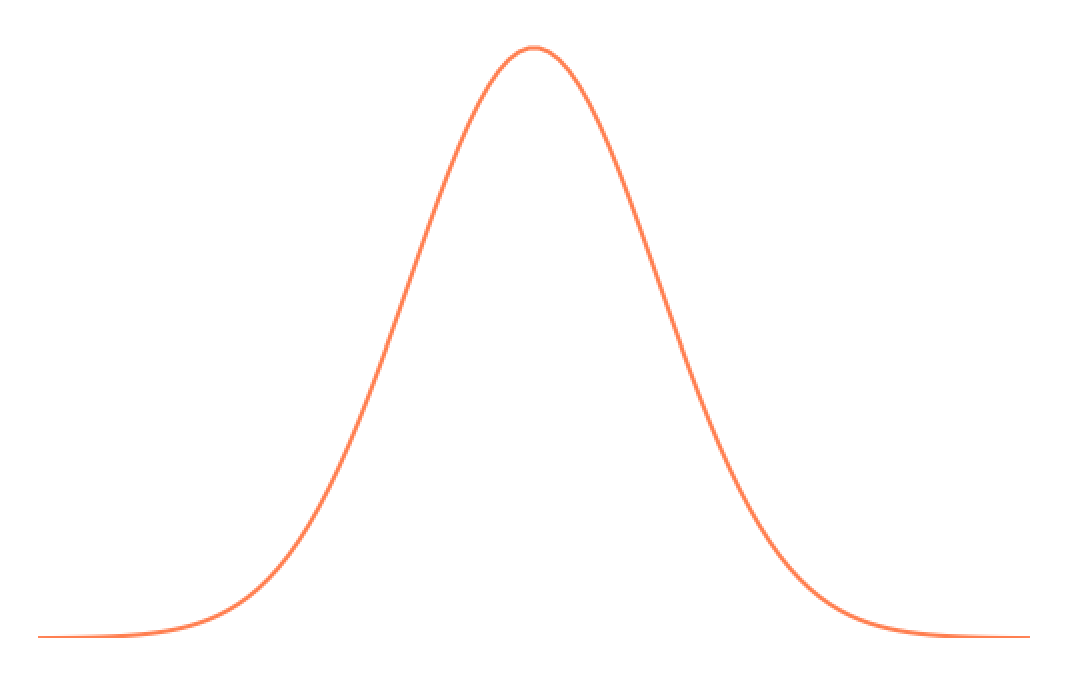
\includegraphics[width=7cm]{figures/normal_dist.png}
    \caption{What a normal distribution looks like.}
    \label{fig:normal_dist_ex}
\end{figure}

The above equation represents a normal distribution, where $\mu$ is the mean of the distribution and $\sigma$ is the standard deviation.

Using R and K in the normal distribution, using equation 1 and 2, we get,

\begin{equation}
    F(x) = \frac{1}{{\frac{1}{K} \sqrt {2\pi } }}e^{{{ - \left( {x - R } \right)^2 } \mathord{\left/ {\vphantom {{ - \left( {x - R } \right)^2 } {\frac{2}{K} ^2 }}} \right. \kern-\nulldelimiterspace} {\frac{2}{K} ^2 }}}
\end{equation}

When initializing the values for the individual infection value, equation 3 is utilized to generate a random normal distribution, while keeping the mean of all the values equal to R while the variance is kept inversely proportional to K. Now this data is used in the algorithm as a metric of how many individual an infected individual can spread the virus to.

\section{Algorithm}
The following depicts and explains the algorithm developed which models the virus spread and simulates it.

Initialization Phase of the algorithm: 
\begin{enumerate}[label=\textbf{\arabic*})]
    \item \textbf{Step 1:} Load the following virus statistics and user specified data mentioned as in section 4.1.
    \begin{enumerate}
        \item R Value
        \item K Value
        \item Infection Range
        \item Mask Effectiveness
        \item Mortality Range
        \item Recovery Time
        \item Population
        \item Healthcare Capacity
        \item Social Distancing Start Time(If Enabled)
        \item Percentage of Individuals Social Distancing(If Enabled)
        \item Mask Mandate Start Time(If Enabled)
    \end{enumerate}
    \item \textbf{Step 2:} Initialize Data
    \begin{enumerate}
        \item Create a matrix where number of rows would be equal to the population with a unique ID for everyone and number of columns is 17 as explained in section 4.1.
        \item Generate a random spread of ages using a continuous uniform distribution\cite{uniform_dist} in a specified range so that they represent a more lifelike age spread.
        \item Generate random starting $(x,y)$ co-ordinates using a continuous uniform distribution for every individual.
        \item Generate random directional $(x,y)$ co-ordinates using a continuous uniform distribution and random wander regions $(x1,x2)$ and $(y1,y2)$ for every individual.
        \item Initialize Individual Infection Value by generating it using a normal distribution which uses R and K values as explained in section 4.2.
        \item Set the speed of movement using a continuous uniform distribution in a specified range for every individual.
        \item Initialize individuals who would be social distancing. Using the percentage specified by the user, random individuals are chosen to participate in social distancing. Social Distancing kicks in after the specified time.
        \item Initialize mask effectiveness for people, if someone would wear a mask and what kind of mask they wear is again decided using a random function. This value would be 0 for individuals not wearing a mask.
        \item Calculate and initialize susceptibility rate for each individual. Susceptibility is calculated by factoring in what kind of mask the individual is wearing and if they're social distancing.
        \item Calculate and initialize mortality chance for each individual. Mortality chances depend upon the individuals age and the viruses mortality rate for that age range.
        \item Choose a random individual, and infect them.
        \item Initialize a integer, $frame = 0$, which will keep track of every single frame/turn in the simulation loop.
    \end{enumerate}
\end{enumerate}

Now entering the looping phase of the algorithm.
\begin{enumerate}[label=\textbf{\arabic*})]
    \item \textbf{Step 1:} 
        
        If $frame ==$ Time at which social distancing starts if enabled:
        
        \hspace{10pt} Start social distancing.
        
        \hspace{10pt} If $frame ==$ Multiple of specified time:
        
        \hspace{20pt} Randomly switch up people following social distancing.
        
    \item \textbf{Step 2:}
    
        If $frame ==$ Time at which mask mandates starts if enabled:
        
        \hspace{10pt} Start mask mandates.
        
    \item \textbf{Step 3:} Move Individuals:
    
        For Individuals who are not deceased and aren't social distancing:
        
        \hspace{10pt} [X co-ordinate value] = [X co-ordinate value] + [Speed]*[X direction value]
        
        \hspace{10pt} [Y co-ordinate value] = [Y co-ordinate value] + [Speed]*[Y direction value]
    
    \item \textbf{Step 4:} Infect People:
    \begin{enumerate}
        \item Find individuals in the infection range for other infected people range whose individual infection value is not 0: 
        \item Infect them based on randomly generated chances using a continuous uniform distribution and their susceptibility.
        \item Decrement individual infection value for individuals who infect others.
    \end{enumerate}
    \item \textbf{Step 5:} Decide outcome:
    \begin{enumerate}
        \item Find infected individuals who have been infected for over the specified recovery time.
        \item Using randomly generated chances using a continuous uniform distribution and their mortality chance decide either they survive for not.
        \item Mark them as immune if they survive, or deceased if they did not.
        \item If the number of currently infected people is extremely above the healthcare capacity at the current moment the chances of an individual dying increases 3 folds.
    \end{enumerate}
    \item \textbf{Step 5:} Update Values for Random Individuals:
    
    Update the directions and speed of 20\% of the population, using a uniform distribution again.
    
    \item \textbf{Step 6:} Check Out of Bounds:
    
    Check if an individual is headed outside of the defined simulation canvas, and chance their directions such that they do not exit the plane.
    
    \item \textbf{Step 7:} $frame = frame + 1$ and jump to \textbf{step 1.}
\end{enumerate}


\section{Output} 
Our GUI looks like the following:

From the configuration screen, we can set following things:
\begin{enumerate}
    \item Population size
    \item Number of people social distancing as a function of the population size
    \item The capacity of the hospital as a function of the population size
    \item The R value for the virus
    \item The K value for the virus
    \item The time social distancing starts (if at all)
    \item The time mask mandate starts (if at all)
    \item Mask effectiveness of 3 types of masks:
    \begin{enumerate}
        \item Cloth masks
        \item Surgical masks
        \item N95 masks
    \end{enumerate}
    \item Mortality rates of 4 age groups:
        \begin{enumerate}
            \item 0-19
            \item 20-49
            \item 50-69
            \item 70+
        \end{enumerate}
\end{enumerate}

Following are a series of screenshots which depict how the GUI looks, and how a user can go around operating the simulation system.
\begin{figure}[H]
    \centering
    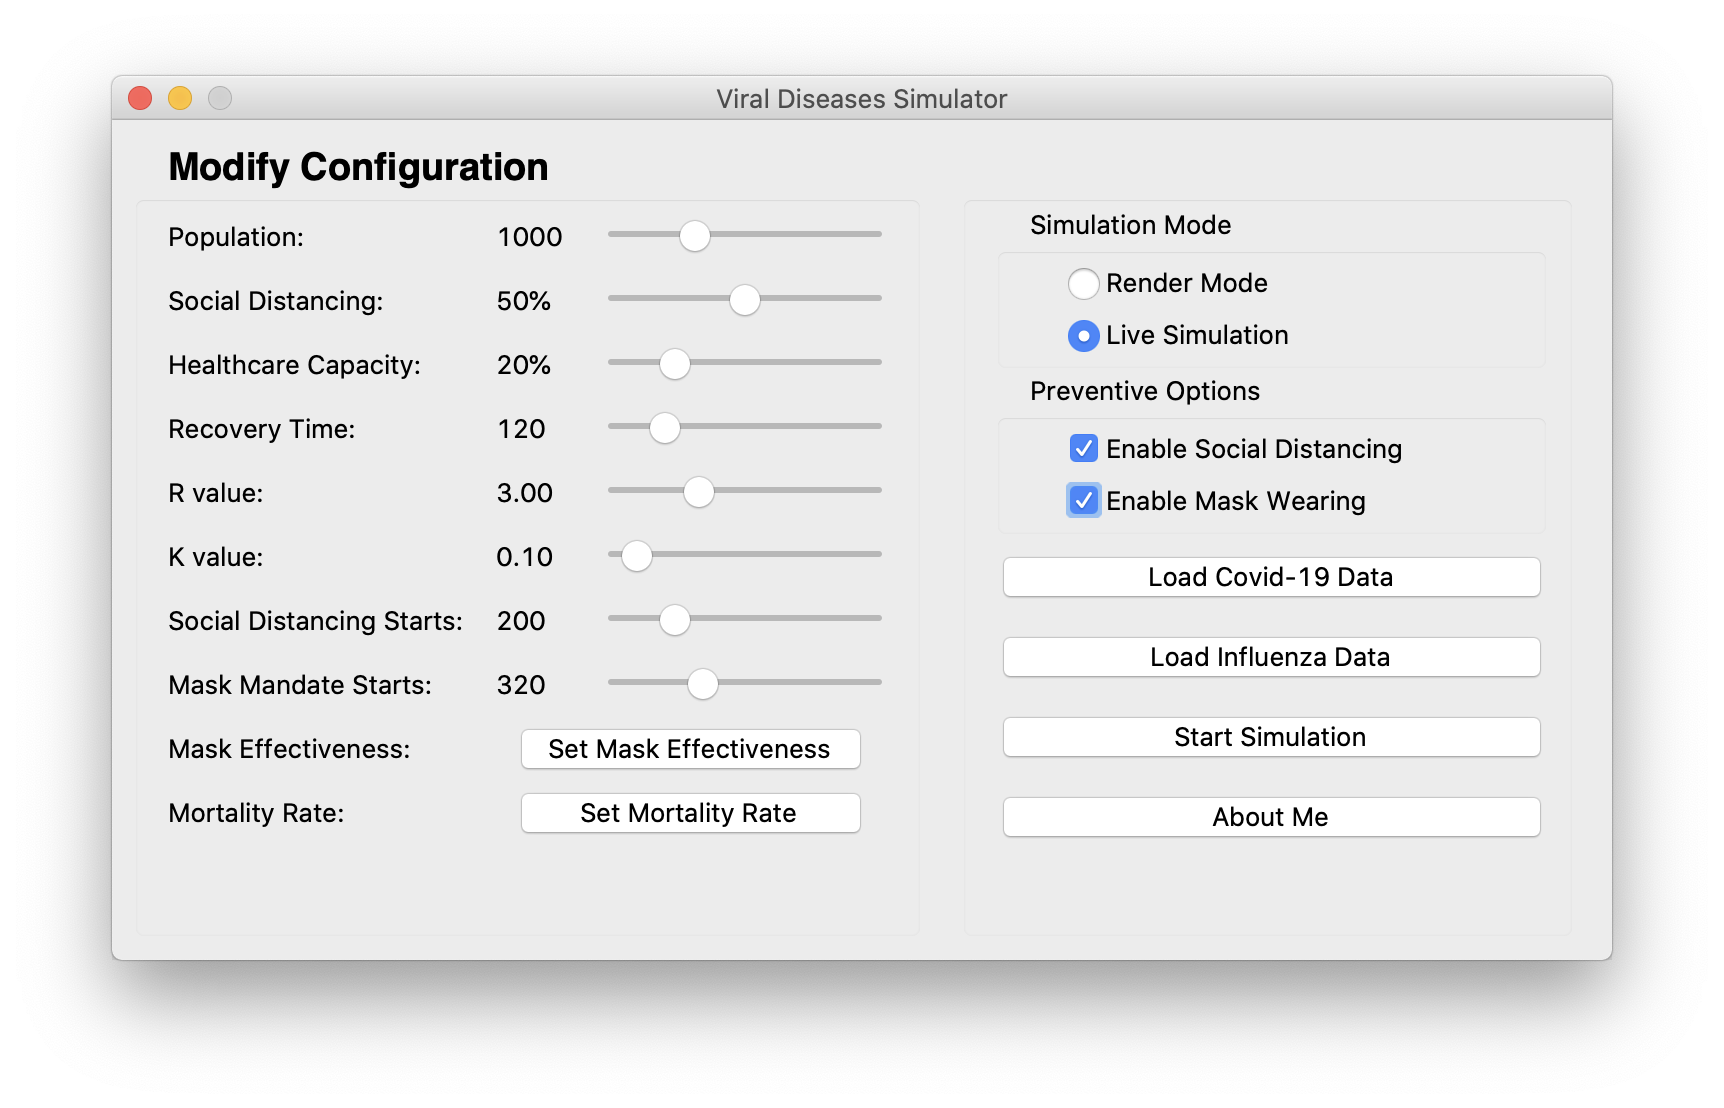
\includegraphics[width=14cm]{figures/ui-vis.png}
    \caption{UI the user is greeted with.}
    \label{fig:main_ui}
\end{figure}
In the figure above, user can click on "Set Mask Effectiveness" button to set how effective different kinds of masks are, or click on "Set Mortality Rate" to set mortality rates for different age groups. User can also enable/disable mask mandates and social distancing using the radio buttons. 

Using the "Load Covid-19 Data" and "Load Influenza Data" button can load the virus statistics to the the program. 

After the user has decided the preferences they want to use, they can decide whether they want to render the simulation to a file or view it live, and then use "Start Simulation" button to initialize the simulation.

\begin{figure}[H]
    \centering
    \begin{subfigure}[b]{0.4\textwidth}
        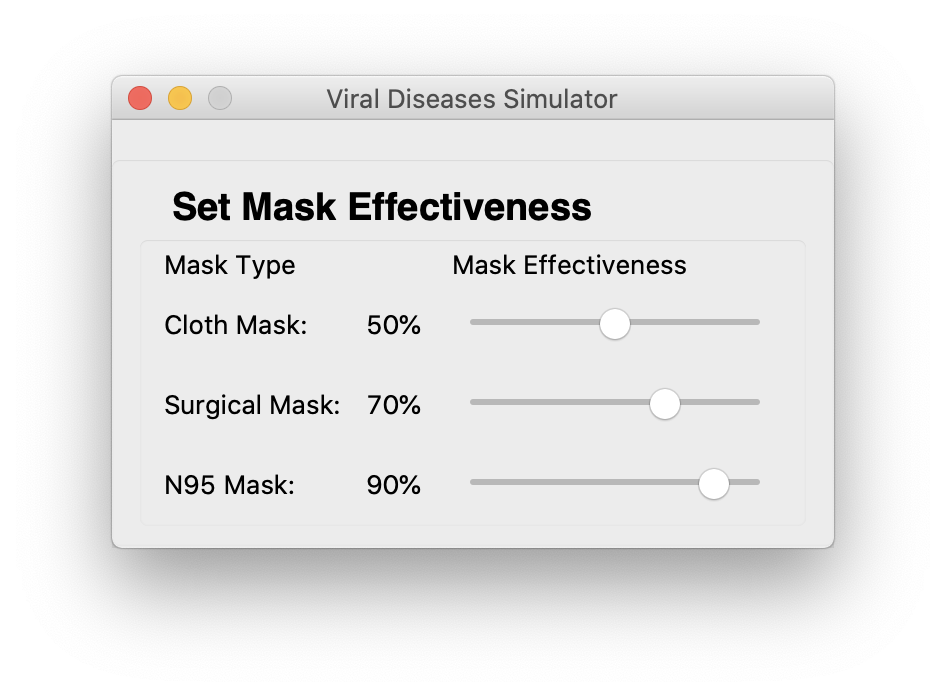
\includegraphics[height=5cm]{figures/GUI-mask.png}
        \caption{Dialog to edit mask effectiveness.}
    \end{subfigure}
    \begin{subfigure}[b]{0.4\textwidth}
        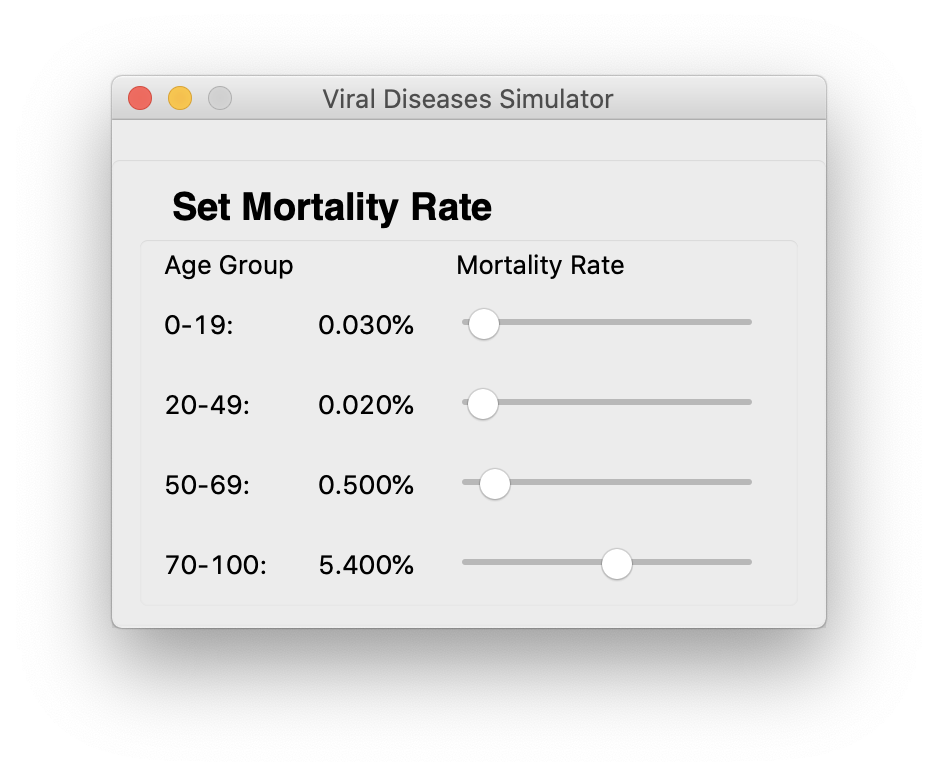
\includegraphics[height=5cm]{figures/GUI-mortality.png}
        \caption{Dialog to edit mortality rate.}
    \end{subfigure}
    \caption{Dialog boxes in the GUI to edit mortality rates and mask effectiveness}
\end{figure}

After clicking on the start button, the user is treated to the following dialog boxes, where the set settings are shown to the user for confirmation before simulation execution. In case the user was in render mode, an additional option for deciding the path to store the render and a disclaimer about additional required libraries and elevated access are shown.

Clicking on start will start the live simulation or the render.
\begin{figure}[H]
    \centering
    \begin{subfigure}[b]{0.4\textwidth}
        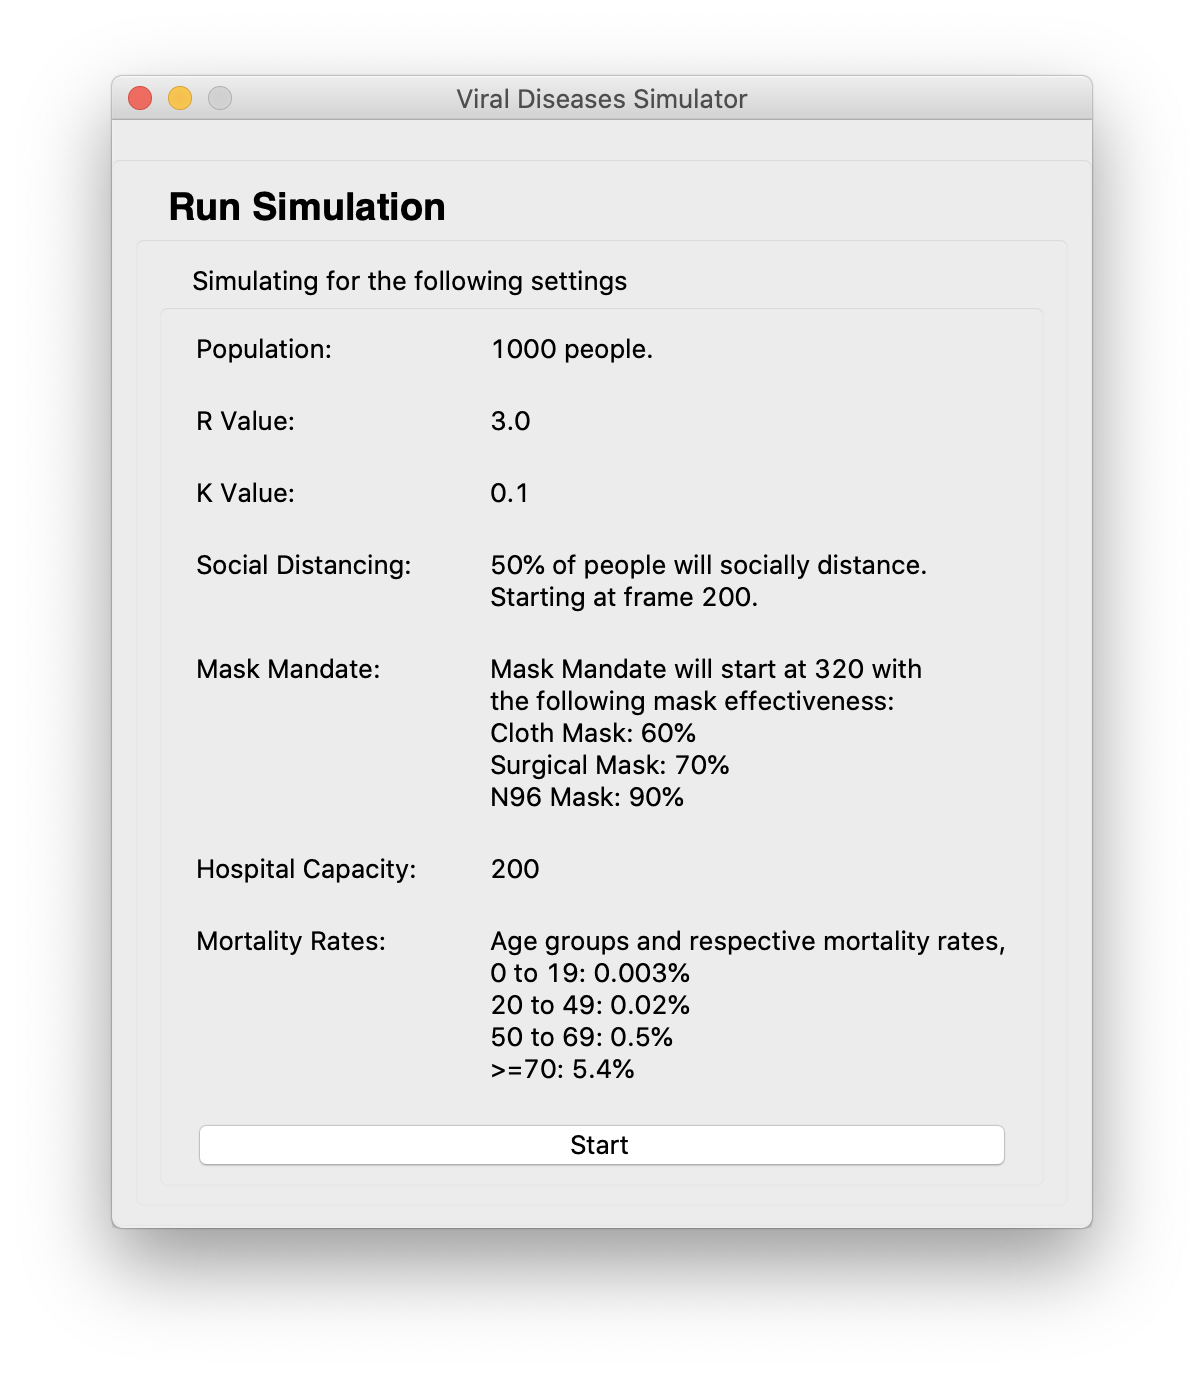
\includegraphics[height=8cm]{figures/GUI-start-sim.png}
        \caption{Start dialog in simulation mode.}
    \end{subfigure}
    \begin{subfigure}[b]{0.4\textwidth}
        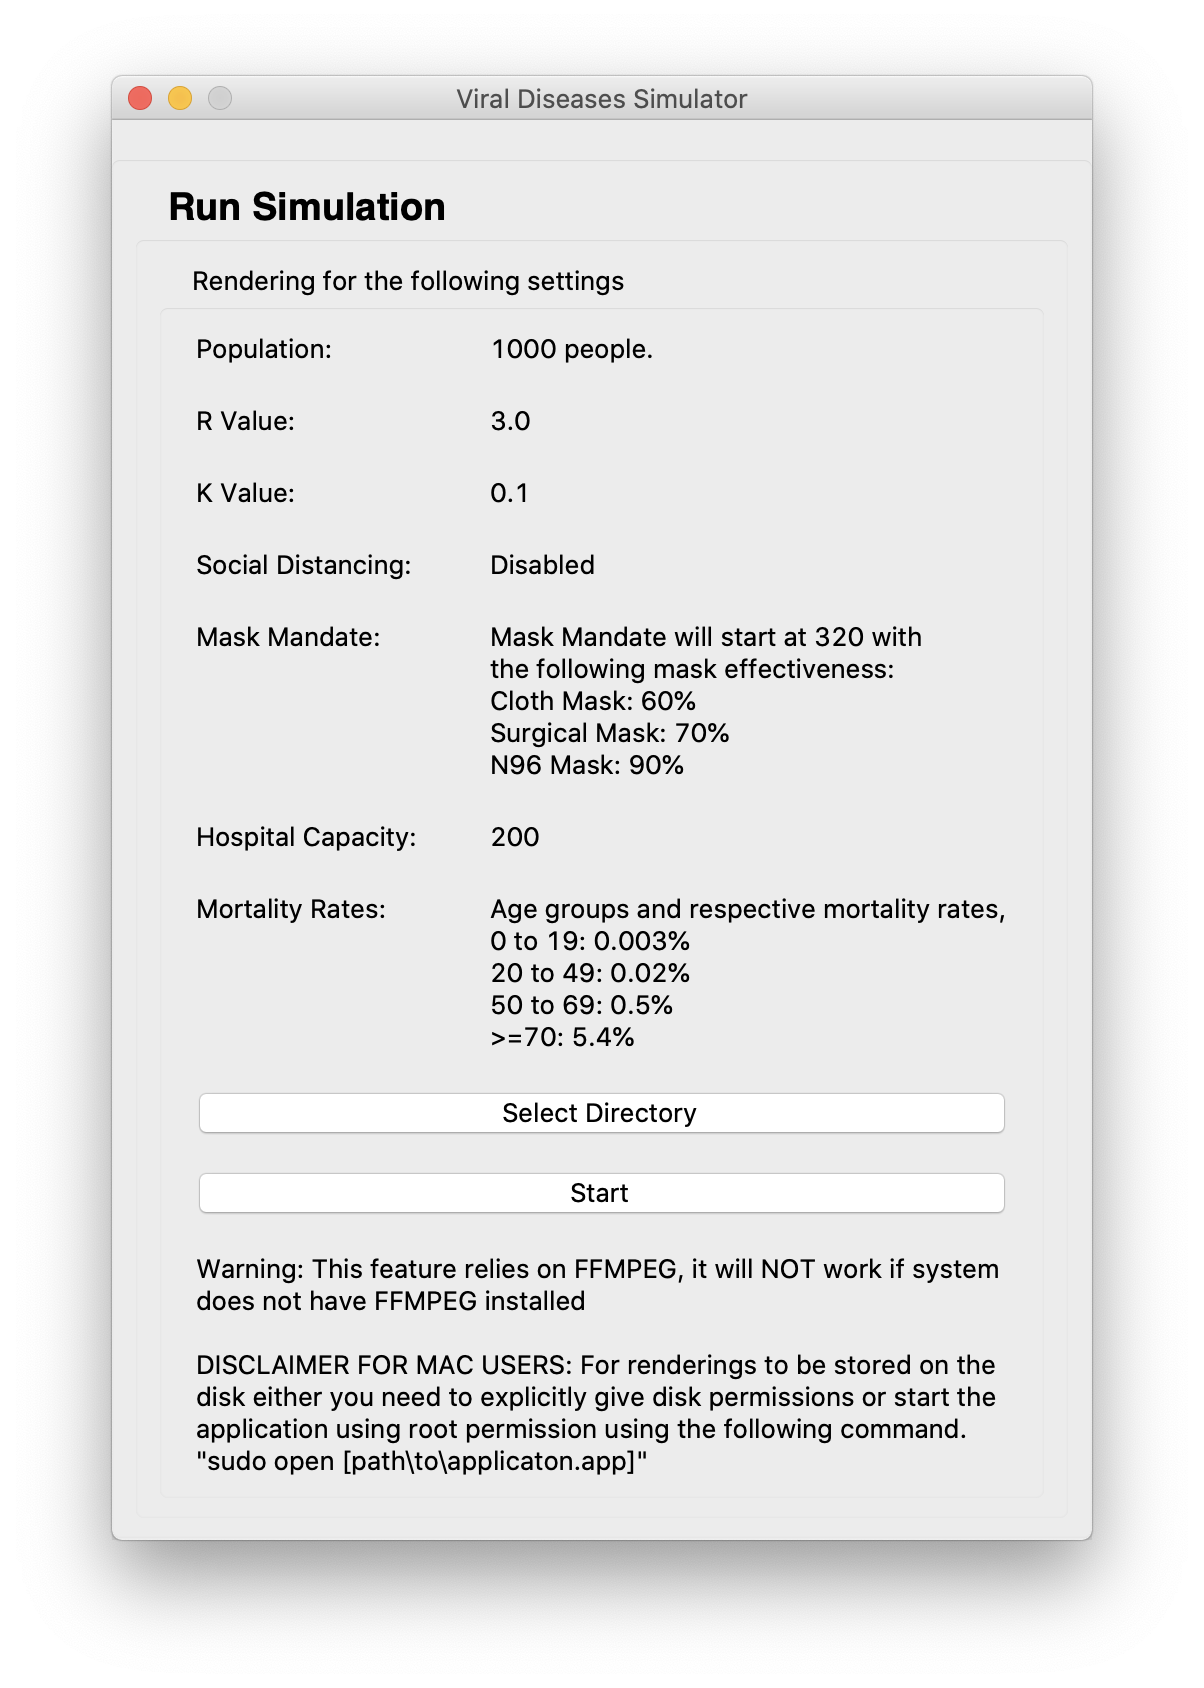
\includegraphics[height=8cm]{figures/GUI-start-ren.png}
        \caption{Start dialog in render mode.}
    \end{subfigure}
    \caption{Dialog boxes when starting simulation.}
\end{figure}
The figure below represents how the simulation either viewed live or rendered looks. The top part of the simulation is a scatter of dots which represent people, with light grey dots representing individuals who are healthy/haven't contracted the virus, orange dots represent individuals who are currently infected, green dots represent individuals who have recovered and are immune, and indigo dots represent individuals who have been deceased.

The middle part of the simulation is a live line graph which depict current trends and data for total number of infected, currently infected, immune and deceased people against time. Vertical lines in the graph depict the time when social distancing or mask mandates start, with yellow representing social distancing and pink representing mask mandates. 

The third and the last part of the simulation show raw statistics of the current simulation, with various data points like population, number and percent of immune and deceased people, when and if preventative measures will start, and how the healthcare conditions are at a given time.

\begin{figure}[H]
    \centering
    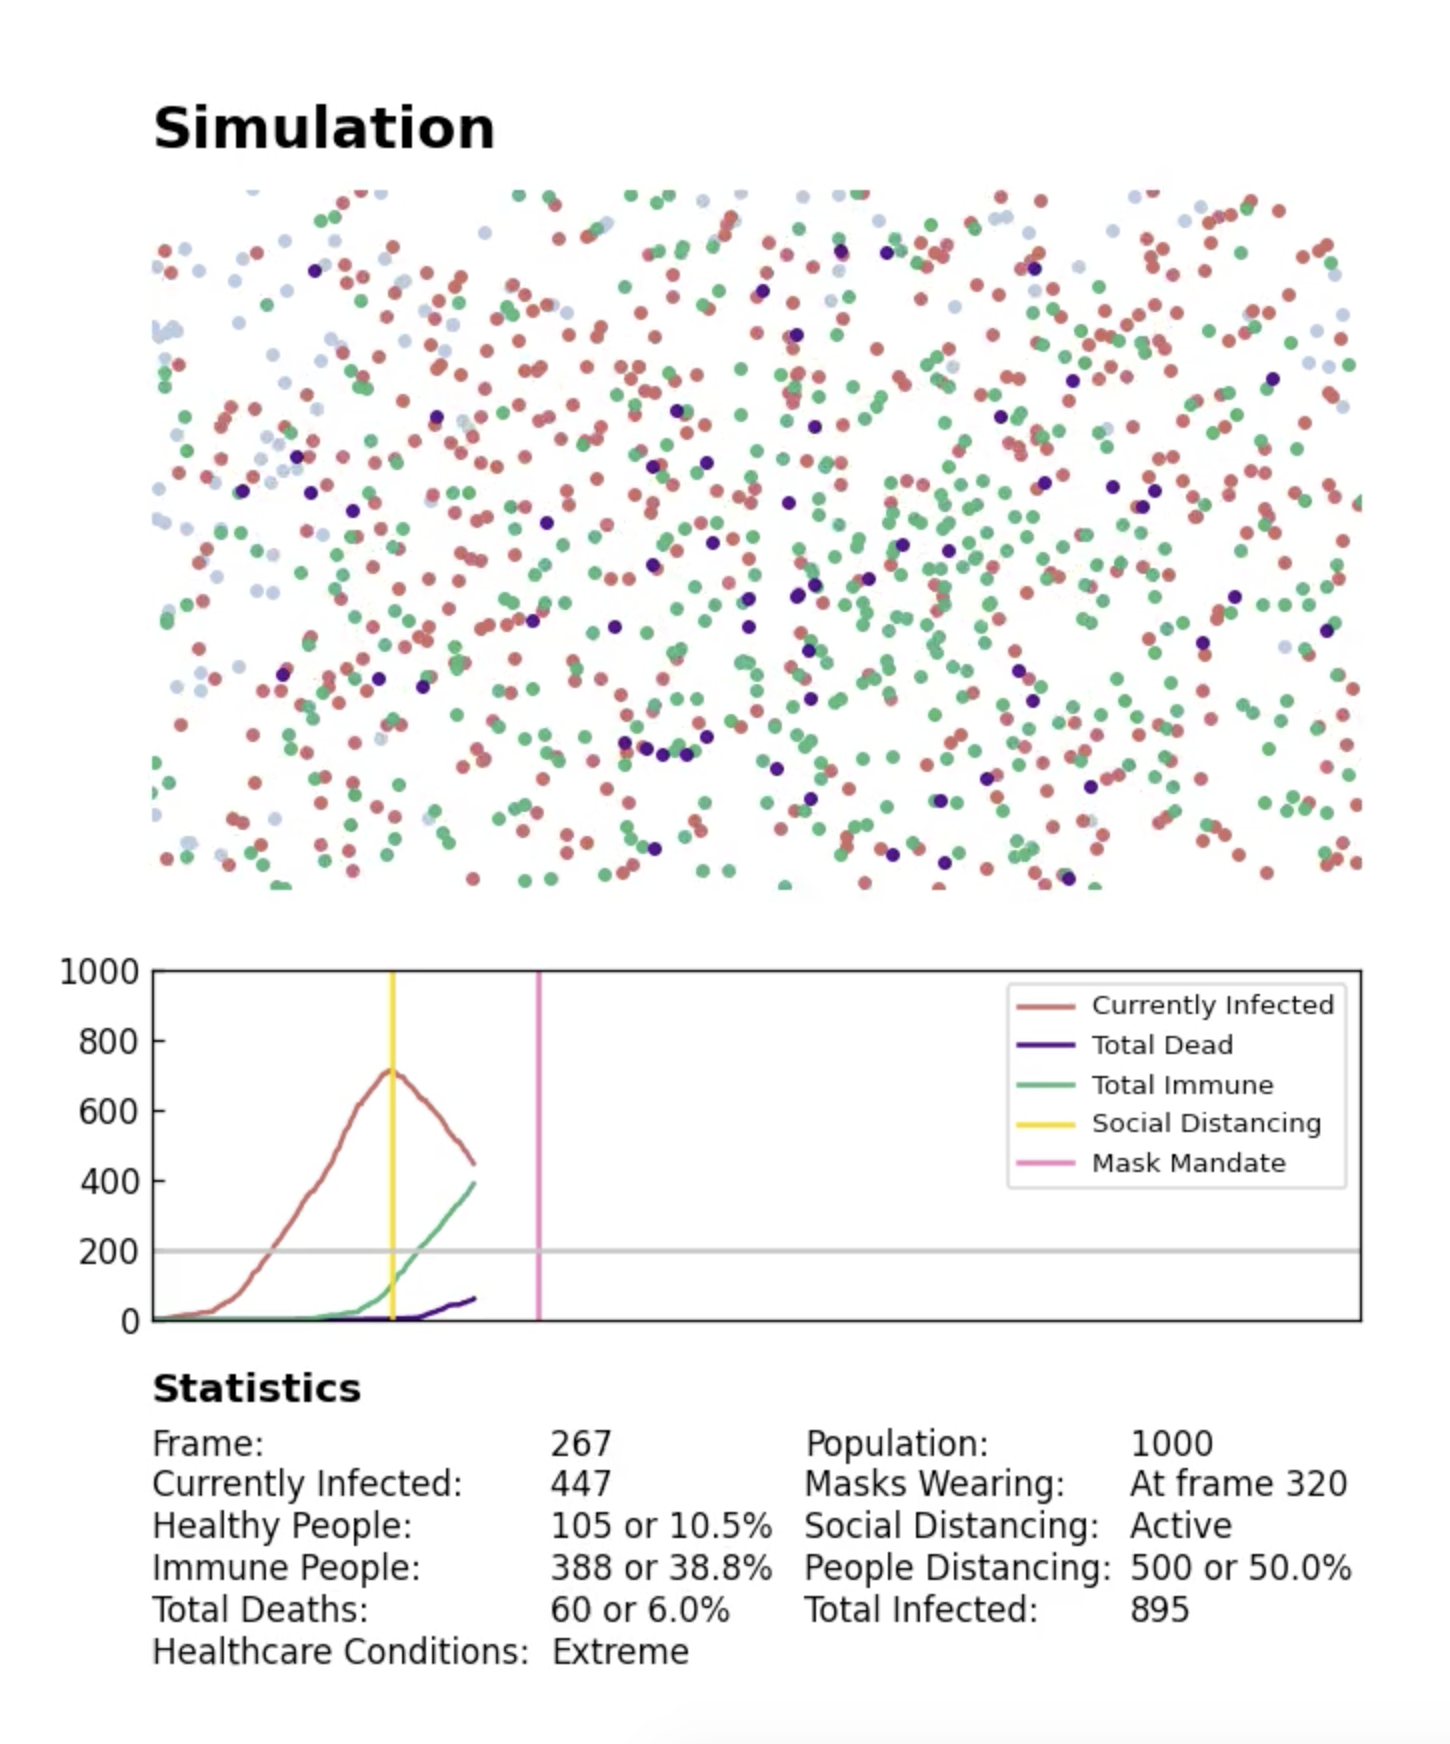
\includegraphics[width=9cm]{figures/simu.png}
    \caption{How the simulation looks.}
    \label{fig:my_label}
\end{figure}
\subsection{Unit Testing}
Unittests have 90\% coverage of the simulation software.

\begin{figure}[H]
    \centering
    \begin{subfigure}[b]{0.45\textwidth}
        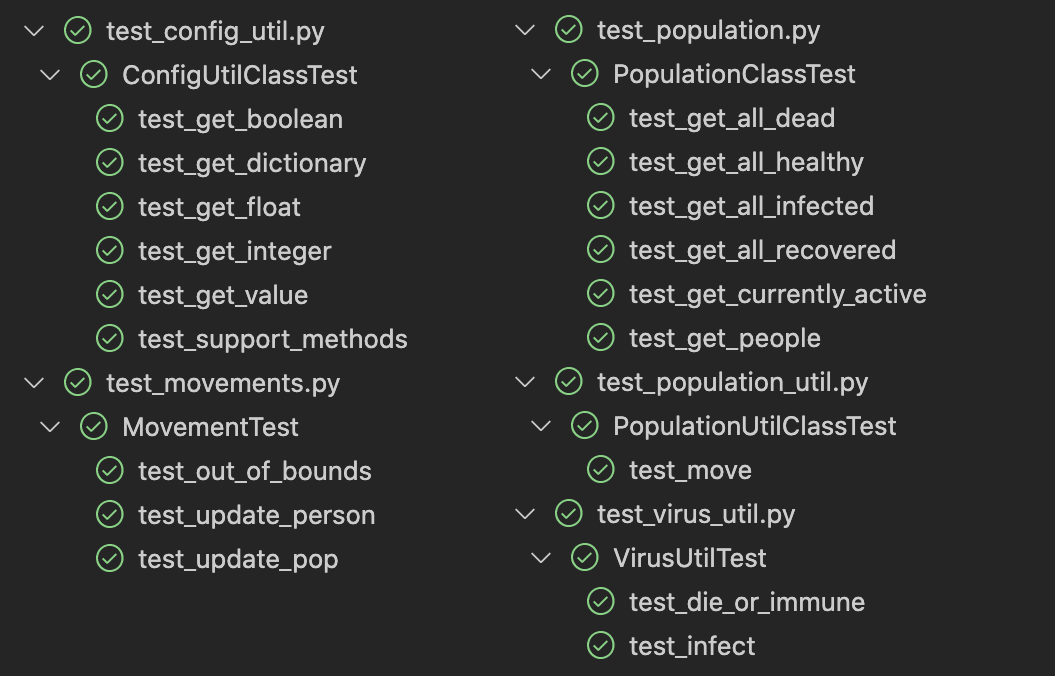
\includegraphics[height=4.5cm]{figures/Tests.png}
        \caption{Screenshot depicting different unittests.}
    \end{subfigure}
    \begin{subfigure}[b]{0.45\textwidth}
        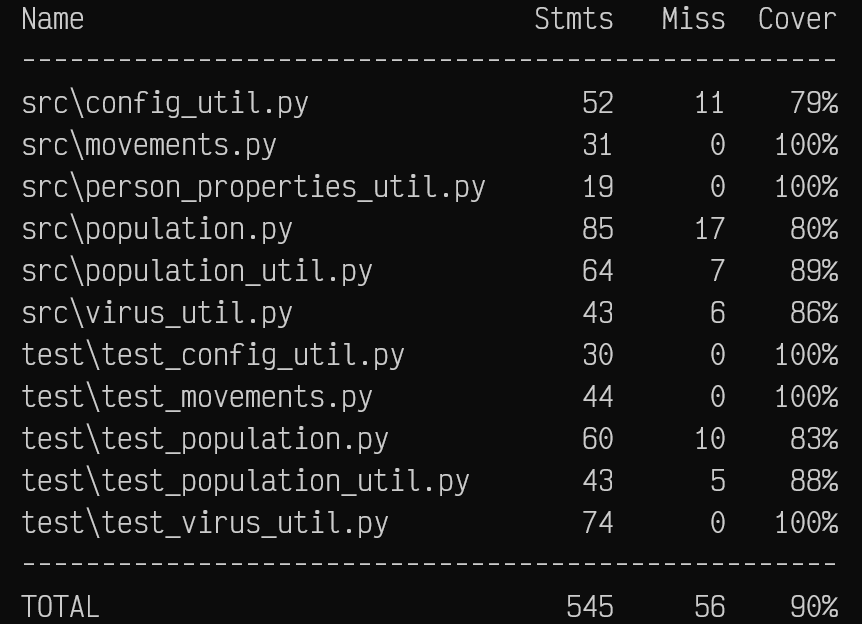
\includegraphics[height=4.5cm]{figures/coverage.png}
        \caption{Screenshot depicting code coverage.}
    \end{subfigure}
    \caption{Screenshots providing insight in unittesting.}
\end{figure}



\section{Mathematical Analysis \& Evidence}

In this section, we explore different factors involved in the spread and impacts of a virus. We vary the factors differently and provide results for each case. We analyze the results are we obtained from our experiment simulations. 

 \subsection{Exponential Growth}
 The exponential growth rate of an outbreak indicates the severeness of the spread of the disease. The growth rate and the reproduction number (R value) are ultimately correlated because with R value greater than 1, the number of infections increase exponentially as each person goes on infect at least 1 person. Once the R value goes below 1, the outbreak slowly starts to contract. This may happen due to two reasons: the entire population gets infected as indicated in  or due to control measures like social distancing and mask mandates taken to reduce the number of people each person goes on to infect. As indicated in Figure \ref{covid-exponential-nomandate} and Figure \ref{covid-exponential-mandates}. 

\begin{figure}[H]
    \centering
    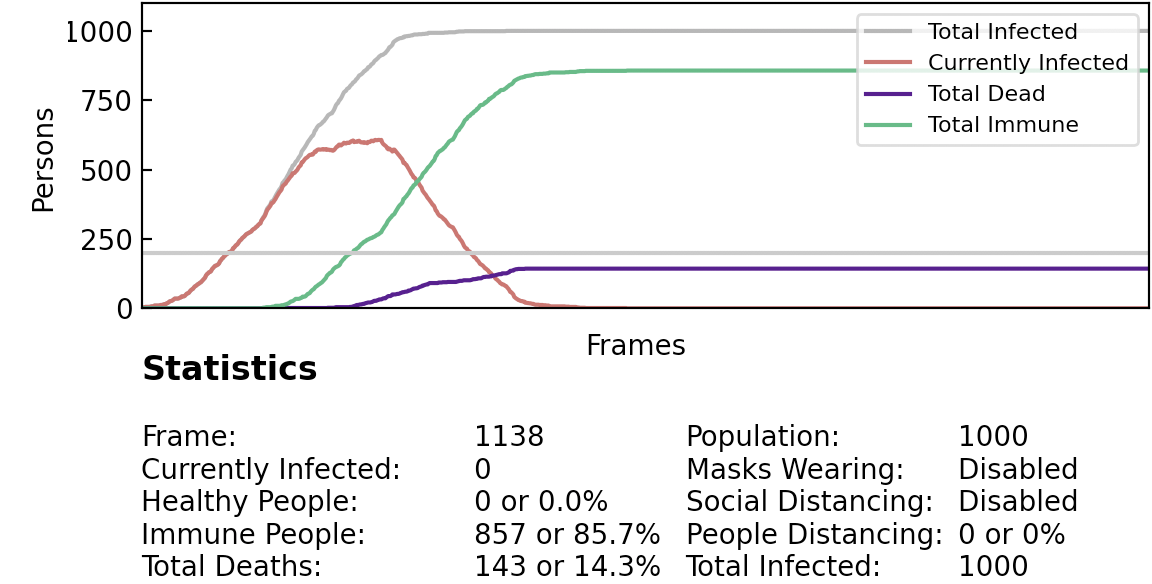
\includegraphics[width=10cm]{figures/covid-nomandates.png}
    \caption{Virus Spread with Time for COVID-19 with no Control Measures}
    \label{covid-exponential-nomandate}
\end{figure}

\begin{figure}[H]
    \centering
    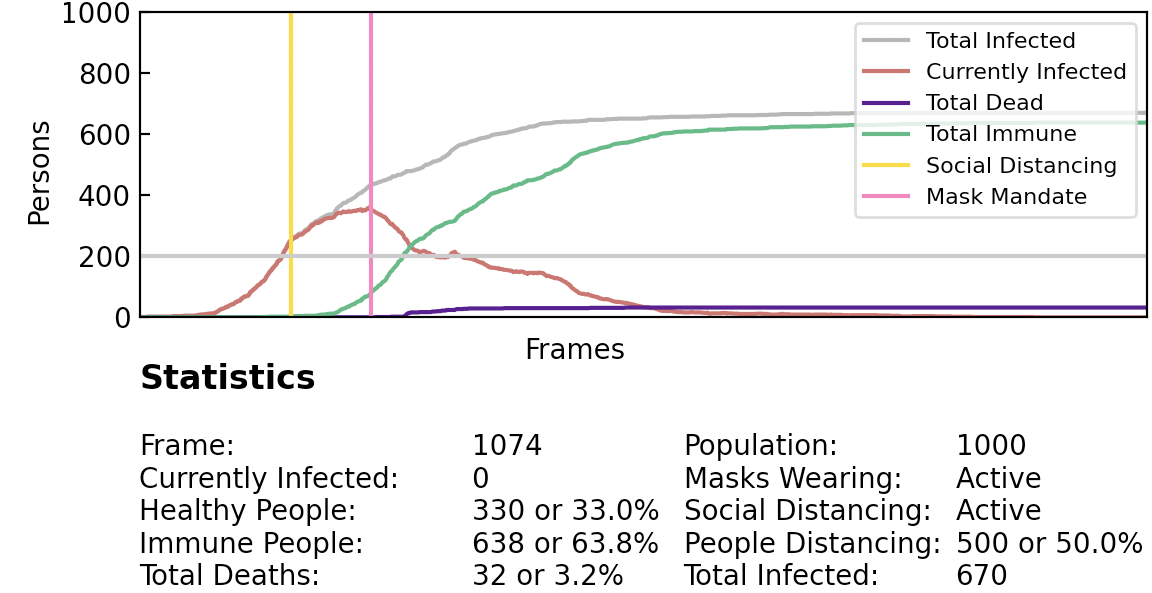
\includegraphics[width=10cm]{figures/covid-propermandates.png}
    \caption{Virus Spread with Time for COVID-19 with Social Distancing and Mask Mandates}
    \label{covid-exponential-mandates}
\end{figure}

In Figure \ref{covid-exponential-nomandate}, one can see that the graph of the total number of total infected grew exponentially and reached a saturation once the entire population had been infected. Meanwhile, in Figure \ref{covid-exponential-mandates}, with social distancing and mask mandate being followed by a percent of the population, the infection grew exponentially, but reached a saturation point at a much lower number with 330 people not catching the disease at all.

\begin{figure}[H]
    \centering
    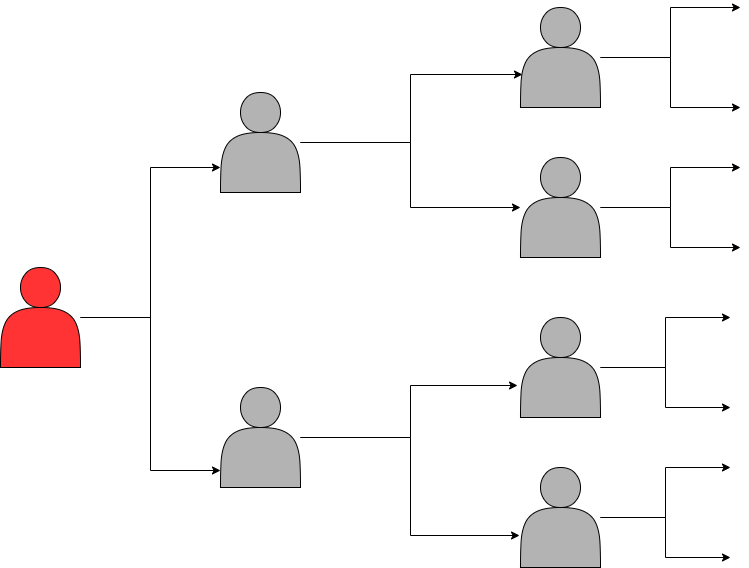
\includegraphics[width=7.5cm]{figures/covid-exponential.png}
    \caption{Assuming a virus with R value of 2, the virus grows exponentially}
    \label{covid-exponential}
\end{figure}

A visual representation of the effects of reproduction number (R value) on how the disease spreads is given in Figure \ref{covid-exponential}. Assuming a virus with R value of only 2, the disease grows exponentially if control measures are not taken.

\subsection{R value} 
As explained in Section 4, the R value indicates the average number of people an infected person goes on to infect. By running a simulation for 3 scenarios: R value equals 1, R value equals to 3 (COVID-19) and R value equals to 8 and keeping all other factors constant one can notice how fast the virus spreads with increasing R value. The simulations for all three cases are shown in Figure \ref{r_value_1}, \ref{r_value_3}, \ref{r_value_8}.

\begin{figure}[H]
    \centering
    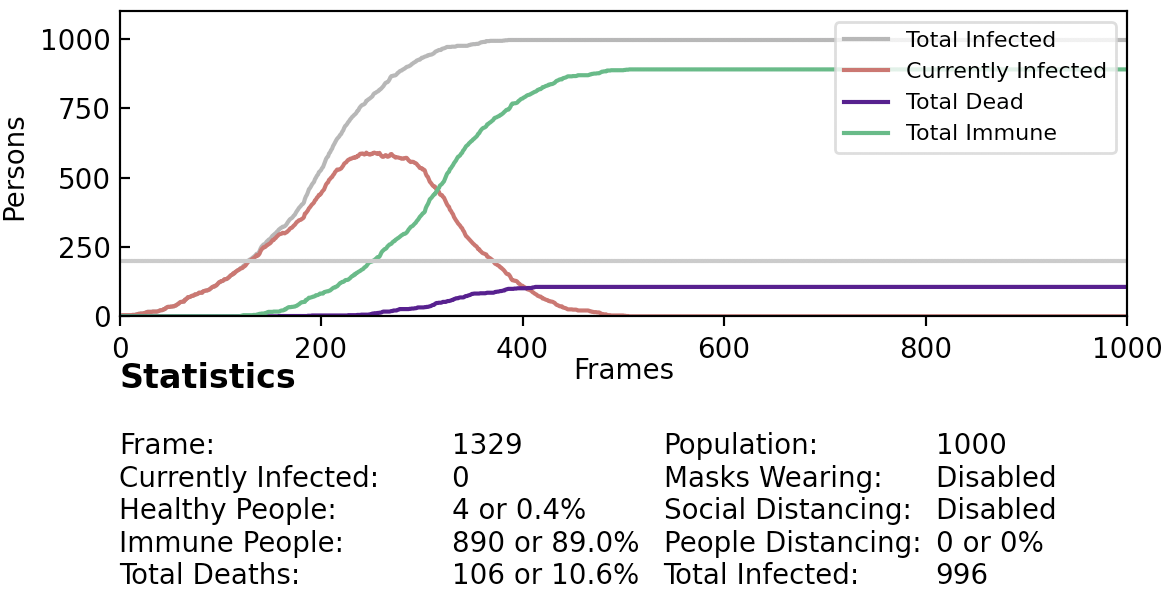
\includegraphics[width=10cm]{figures/r_value_comparison1.png}
    \caption{Virus Spread with Time when R value = 1 and K value = 1}
    \label{r_value_1}
\end{figure}

\begin{figure}[H]
    \centering
    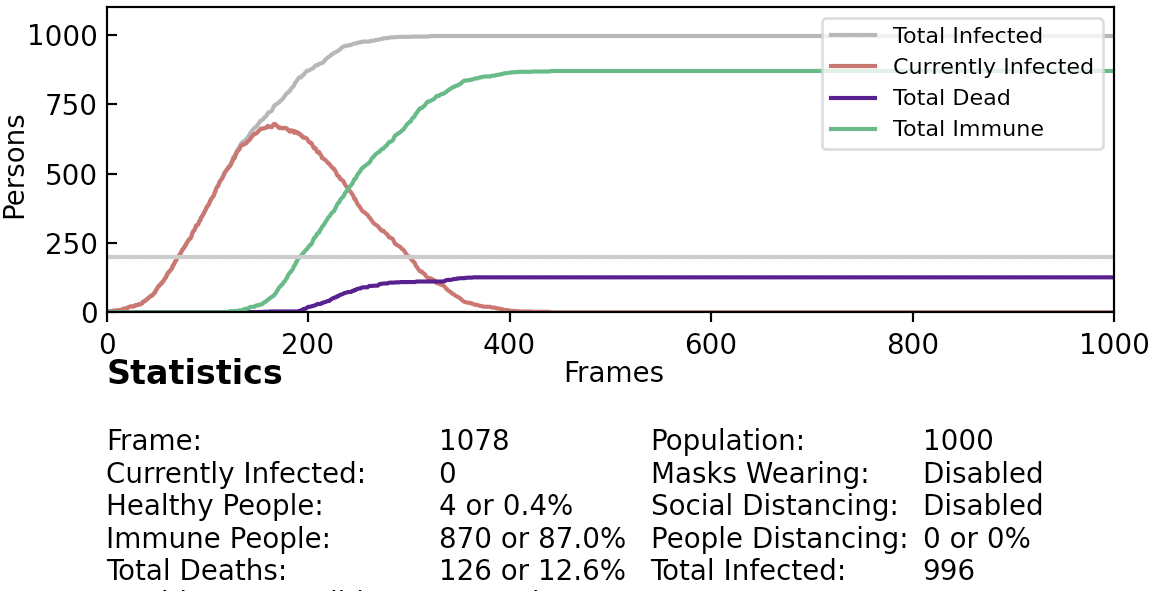
\includegraphics[width=10cm]{figures/r_value_comparison3.png}
    \caption{Virus Spread with Time when R value = 3 and K value = 1}
    \label{r_value_3}
\end{figure}

From the shown graphs, one can see that for R = 1, the virus was spread much slower than for higher R values with the peak current infection rate being observed at roughly 250$^\text{th}$ frame. The curve for currently infected is also much more spread out meaning that the healthcare facility capacity is not overwhelmed all that much, thereby causing lower number of deaths. The number of deaths in these scenario was only 106 (10.6\%) people. This is also known as flattening the curve, a common term being used these days to promote control measures amongst the population so as to not let healthcare facility capacity reach its limit. 

For R = 3, the curve is spread out although not as much as for R = 1 and the peak is reached around 200$^\text{th}$ frame. The number of deaths in this scenario is 126 (12.6\%) people.

\begin{figure}[H]
    \centering
    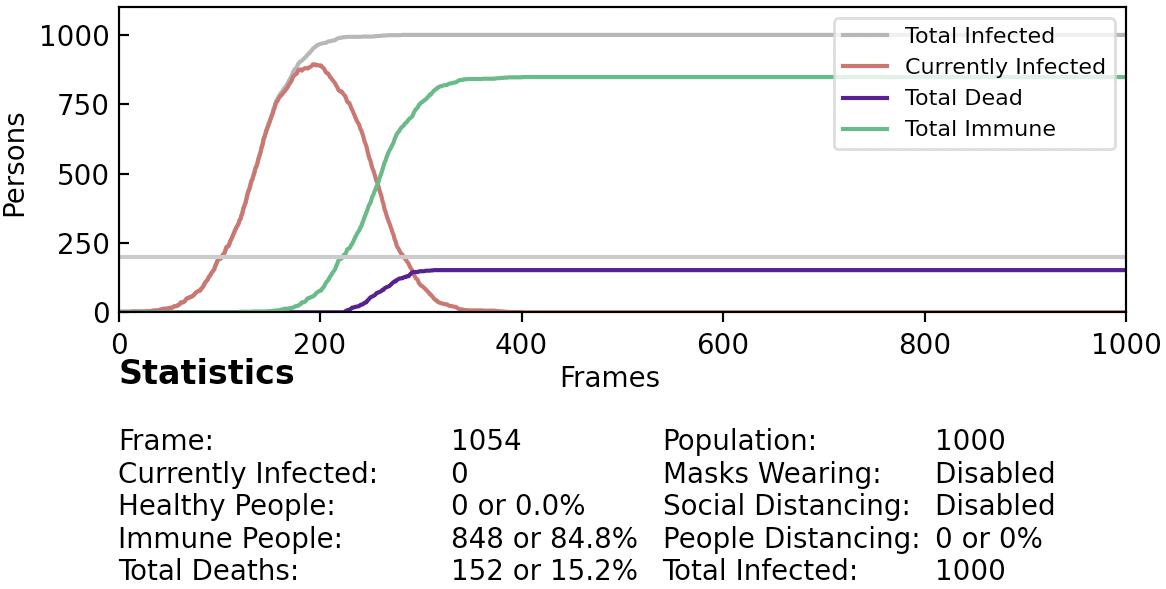
\includegraphics[width=10cm]{figures/r_value_comparison8.png}
    \caption{Virus Spread with Time when R value = 8 and K value = 0.1}
    \label{r_value_8}
\end{figure}

For R = 8, the peak is observed way earlier and there comes a point where barely anyone has recovered but the entire population has already contracted the disease. The peak for the currently infected is higher, steeper and reached before the 200$^\text{th}$ frame. This is an extremely devastating scenario for the healthcare facilities as they are much more likely to run out of ICUs and hospital beds causing a higher number of deaths. The number of deaths observed in this scenario is the highest i.e 152 people (15.2\%) which is to be expected. We can conclude that faster the infection spreads, the more likely it is to cause a large number of spreads as hospitals are not able to accommodate every person who may require healthcare facilities. 

\subsection{K value}
As also explained in Section 4, K value is the dispersion of individual reproduction value of the virus for a person. For lower K values, the variance is much higher, thereby a person is more likely to either not spread the disease at all or cause superspreader events. Hence, for lower K values, one would expect more superspreader events and faster exponential growth as compared to higher K values for which the the infection curve would be more spread out. Our experiment simulation results can be seen in Figure \ref{k_value_3} and \ref{k_value_0.03}.

\begin{figure}[H]
    \centering
    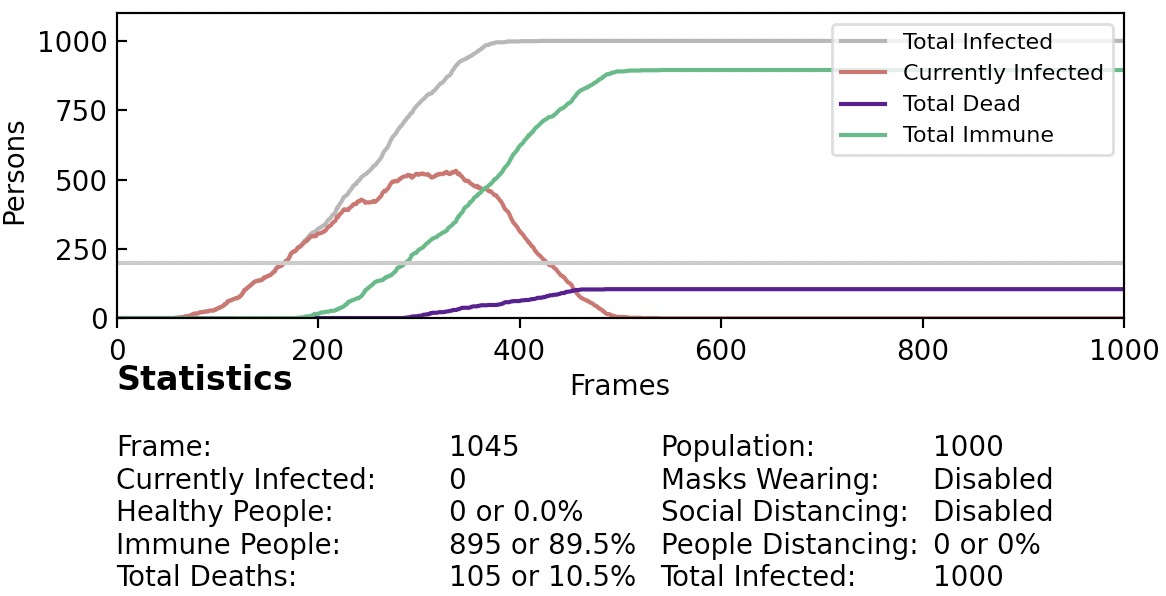
\includegraphics[width=10cm]{figures/k_value_comparison_3.png}
    \caption{Virus Spread with Time when K value = 3 and R value = 3}
    \label{k_value_3}
\end{figure}

\begin{figure}[H]
    \centering
    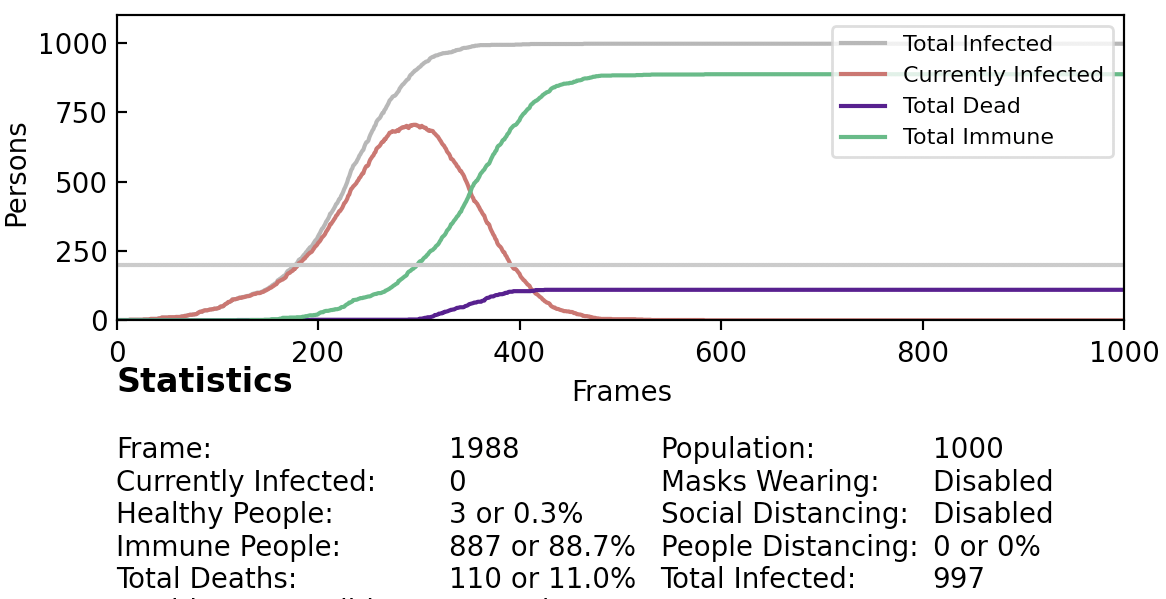
\includegraphics[width=10cm]{figures/k_value_comparison_0.03.png}
    \caption{Virus Spread with Time when K value = 0.03 and R value = 3}
    \label{k_value_0.03}
\end{figure}

One can observe that for K value = 0.03, the curve for current infections was steeper while for K = 3, the curve for current infections was much more spread out. This indicates that when K value is lower, there are more chances of superspreader events causing faster exponential growth.

\subsection{Social Distancing} 
With the spread of COVID-19, each country, even each town had different responses to the pandemic. From the data emerging from different areas showing the virus demonstrating different growths
one cannot stress enough the importance that social distancing has played in maintaining and reducing the virus spread. However, there are two main factors that come into play when one talks about how useful social distancing has been. These factors are mainly how soon the advisory was put into place and the percentage of the population that is social distancing\cite{social_distancing}. We discuss the impact of social distancing in two different cases: 
\begin{enumerate}
    \item \textbf{How early social distancing was put into place}: We run 3 different experiments for social distancing during COVID-19: No social distancing put into place, social distancing implemented at an earlier stage of the outbreak, social distancing implemented at a later stage of the outbreak. In the latter two cases, 50\% of the population is social distancing. Our results our reported in Figure \ref{no_social_distancing}, \ref{social_distancing_150}, \ref{social_distancing 300}.
    \begin{figure}[H]
    \centering
    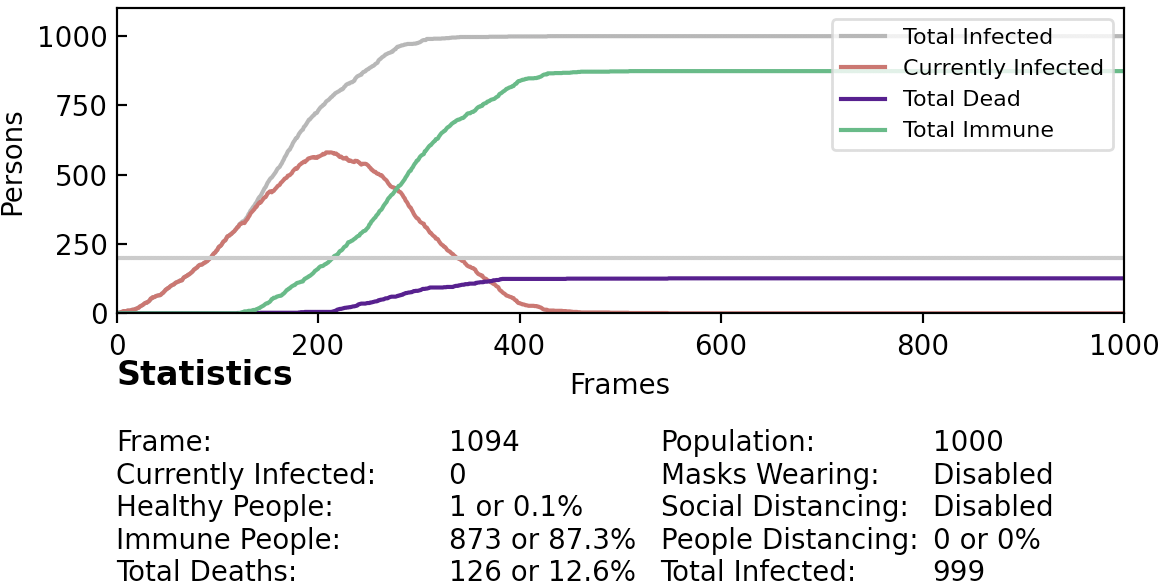
\includegraphics[width=10cm]{figures/no_social_distancing.png}
    \caption{Virus Spread with Time for COVID-19 with No Social Distancing}
    \label{no_social_distancing}
\end{figure}

\begin{figure}[H]
    \centering
    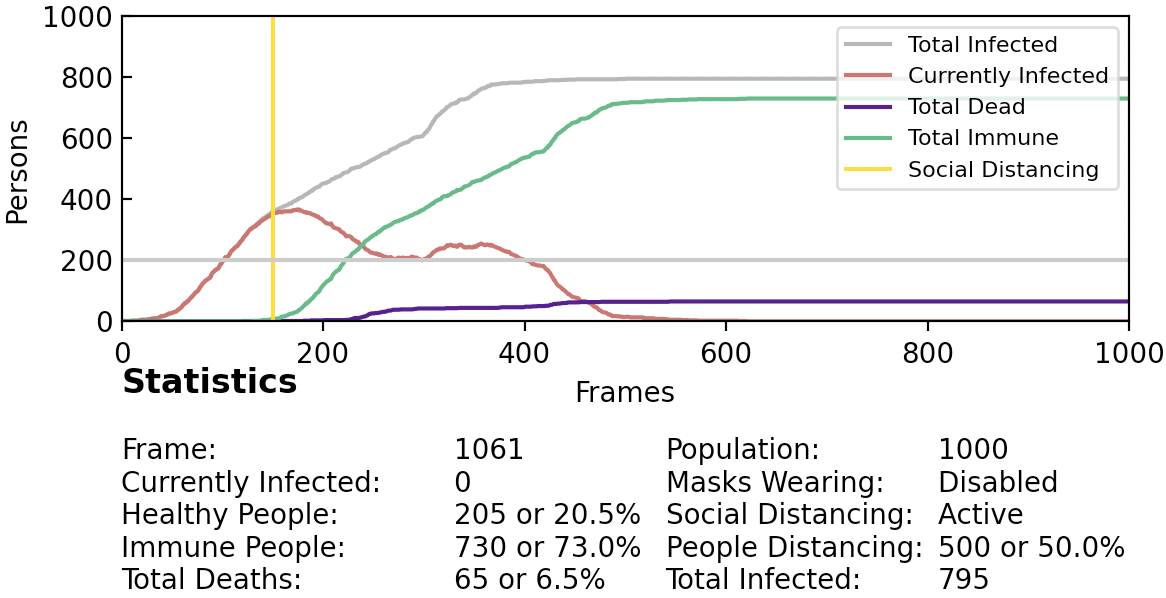
\includegraphics[width=10cm]{figures/social_distancing_150.png}
    \caption{Virus Spread with Time for COVID-19 with 50\% of the Population Social Distancing starting at Frame 150}
    \label{social_distancing_150}
\end{figure}

\begin{figure}[H]
    \centering
    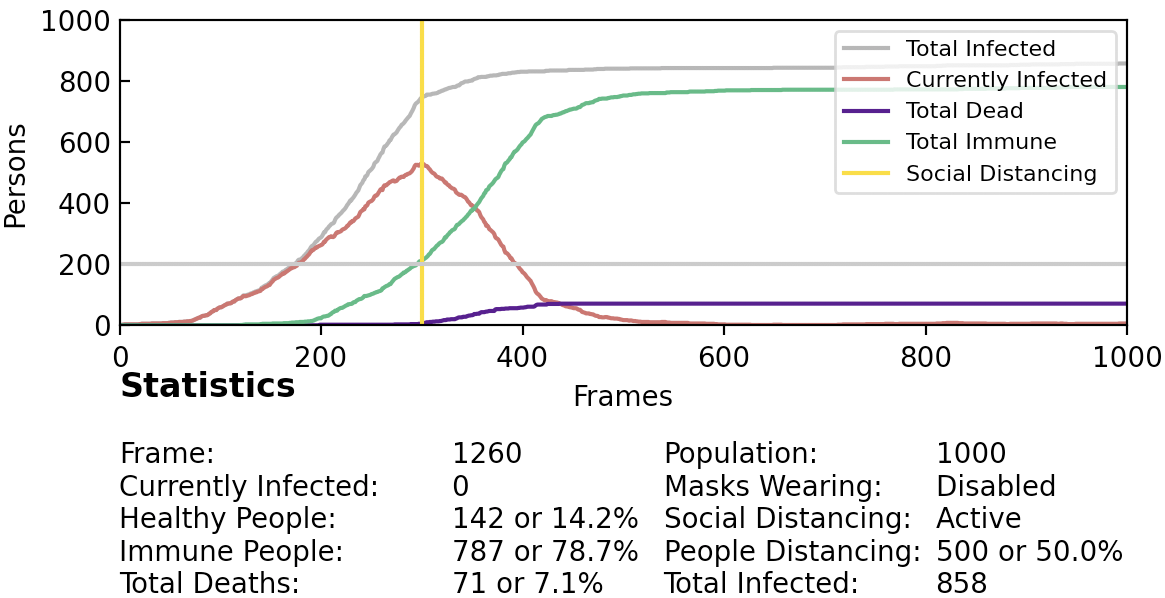
\includegraphics[width=10cm]{figures/social_distancing_300.png}
    \caption{Virus Spread with Time for COVID-19 with 50\% of the Population Social Distancing starting at Frame 300}
    \label{social_distancing 300}
\end{figure}

In Figure \ref{no_social_distancing}, where no one socially distances at all, we observe that the virus grows exponentially until all the population has contracted the disease. 126 (12.6\%) people died in this case and the entire population got the virus. 


In Figure \ref{social_distancing_150}, where social distancing starts at an early stage (150$^\text{th}$ frame), one can see that at one point, at most only 400 (40.0\%) people were infected which greatly impacted the death rates as only 65 (6.5\%) people died in this case. This happened because the healthcare facilities were not overwhelmed by the surge of cases at once and thereby could admit the people who required hospitalizations, thereby reducing the morbidity of the virus. Total number of infections in this case was only 795 (79.5\%) people.


In Figure \ref{social_distancing 300}, one can see that once social distancing advisory was put into place even at a later stage (300$^\text{th}$ frame), the number of current infections started declining almost immediately. With 858 (85.8\%) total infections and 71 (7.1\%) deaths even with the advisory implemented at a later stage, it is easy to tell how important social distancing is when it comes to controlling the outbreak.

\item \textbf{Percentage of people social distancing}: We run 3 different experiments for social distancing during COVID-19: 20\% of the population is social distancing, 50\% of the population is social distancing, 80\% of the population is social distancing. In all these experiments, social distancing starts at Frame 200. Our results are reported in \ref{social_distancing_20percent}, \ref{social_distancing_50percent}, \ref{social_distancing_80percent}

    \begin{figure}[H]
    \centering
    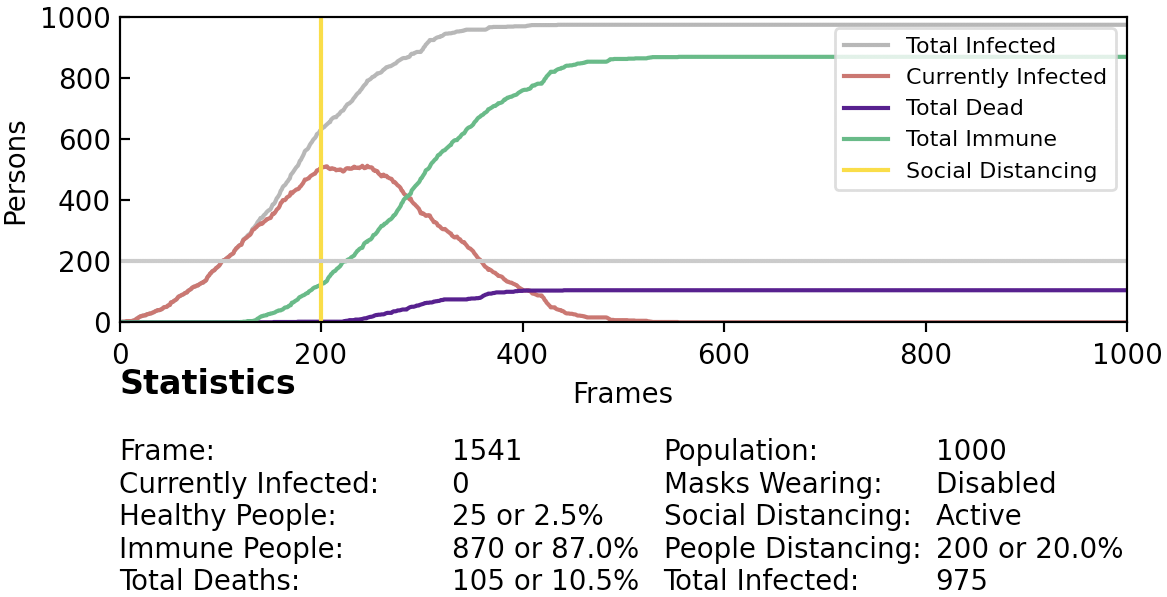
\includegraphics[width=10cm]{figures/social_distancing_20percent.png}
    \caption{Virus Spread with Time for COVID-19 with 20\% of the Population Social Distancing at Frame 200}
    \label{social_distancing_20percent}
\end{figure}

\begin{figure}[H]
    \centering
    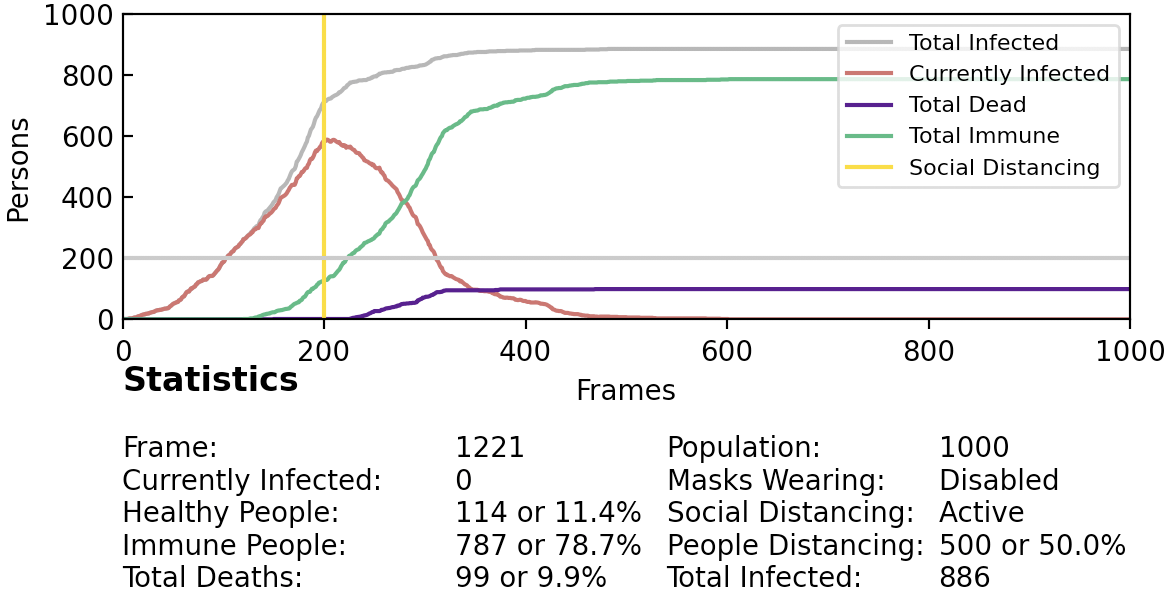
\includegraphics[width=10cm]{figures/social_distancing_50percent.png}
    \caption{Virus Spread with Time for COVID-19 with 50\% of the Population Social Distancing at Frame 200}
    \label{social_distancing_50percent}
\end{figure}

\begin{figure}[H]
    \centering
    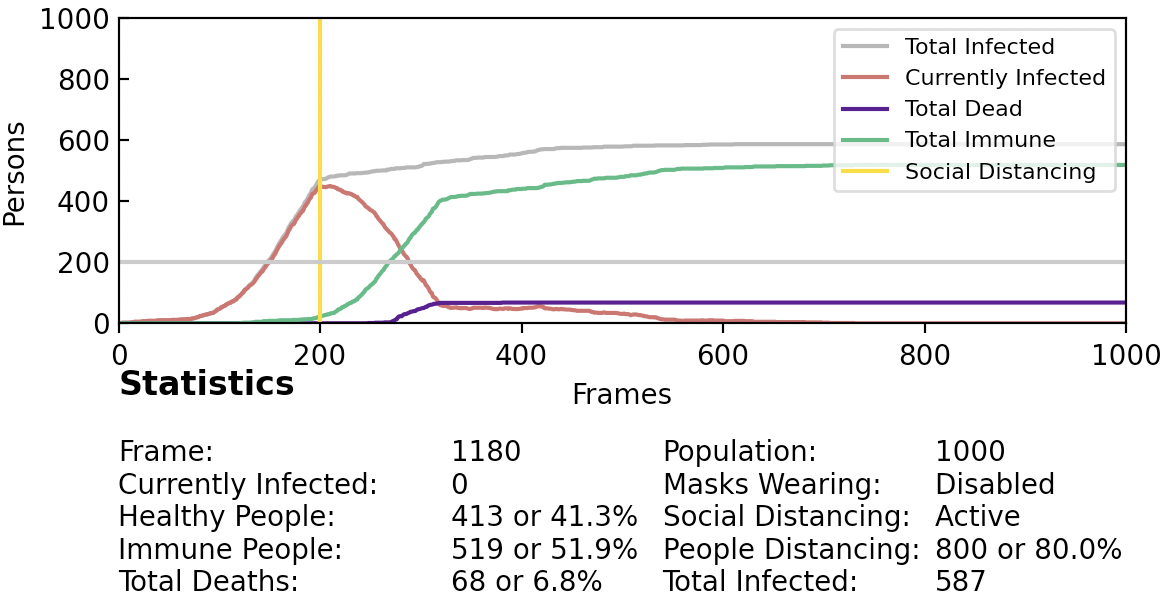
\includegraphics[width=10cm]{figures/social_distancing_80percent.png}
    \caption{Virus Spread with Time for COVID-19 with 80\% of the Population Social Distancing at Frame 200}
    \label{social_distancing_80percent}
\end{figure}

In Figure \ref{social_distancing_20percent}, we can see that since only 20\% of the population was social distancing, the infection curve was spread out but that did not stop the infection from spreading to the entire population. This implies that 20\% of the population social distancing is not enough to control the outbreak. This scenario demonstrates the highest number of deaths i.e 105 (10.5\%).


In Figure \ref{social_distancing_50percent}, there is slight improvement from the above case, where a larger section of the population never contracted the virus at all i.e 114 people (11.4\%). This can be attributed to 50\% of the population social distancing. The total deaths in this case were also lower in comparison i.e 99 (9.9\%). 

In Figure \ref{social_distancing_80percent}, we see the best results, where a big section of the population never contracted the virus at all i.e 587 people (58.7\%). This can be attributed to 80\% of the population social distancing. The total deaths in this case were the lowest i.e 68 (6.8\%). This goes on to show that outbreak control is possible if a larger than half of the population social distances.
\end{enumerate}

\subsection{Population Density}
Population density plays a role in how fast the virus spreads. When people are sparsely located, they are less likely to come in contact with an infected individual\cite{density}. When they are located in a more dense area, the virus spreads much faster as the probability of a healthy individual coming in contact with an infected person increases. There have been contradicting studies specific to COVID-19 that suggest that population density may not be linked to higher density if the activity in the population is low \cite{covid_lowdeath}\cite{covid_urban}. These studies are based on real urban settings with some sort of social distancing and mask mandates already in place. However, in our experiments, since there are no control measures in place to reduce activity/movement, the virus spreads faster. To show this, we run three simulation experiments for COVID-19: a population consisting of only 500 people, 1000 people, and 3000 people while keeping the size of the area and all the other factors the same. Here we see how fast the virus spreads for all 3 scenarios. The results are reported in Figure \ref{population_denisty_522}, \ref{population_density_1000}, \ref{population_density_3000}. 

 \begin{figure}[H]
    \centering
    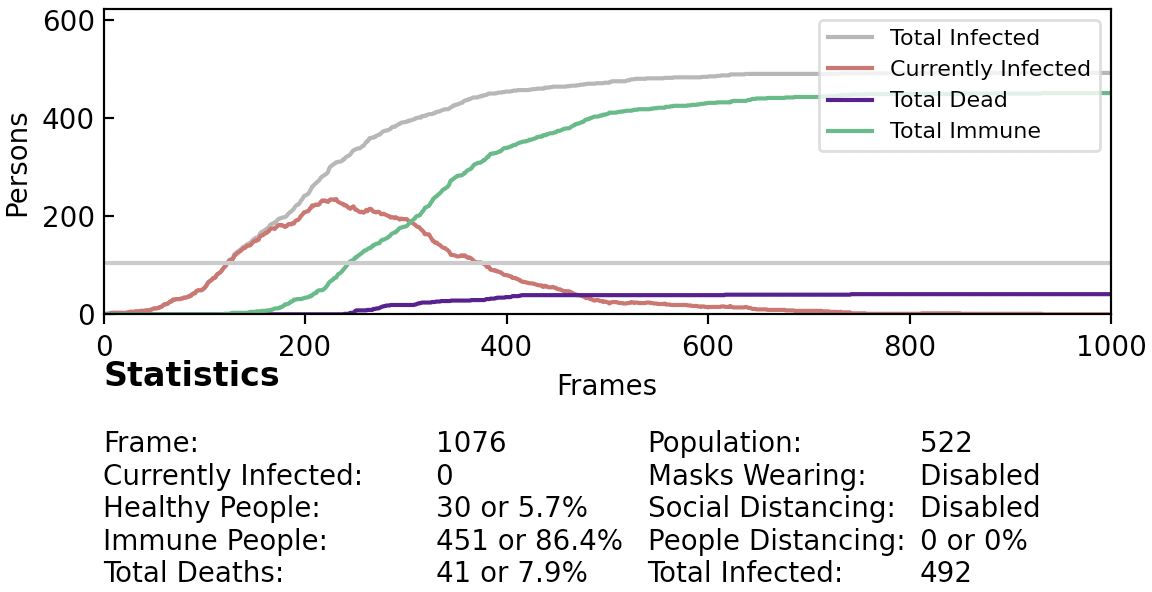
\includegraphics[width=10cm]{figures/population_denisty_522.png}
    \caption{Virus Spread with Time for COVID-19 with Population Size = 522}
    \label{population_denisty_522}
\end{figure}

\begin{figure}[H]
    \centering
    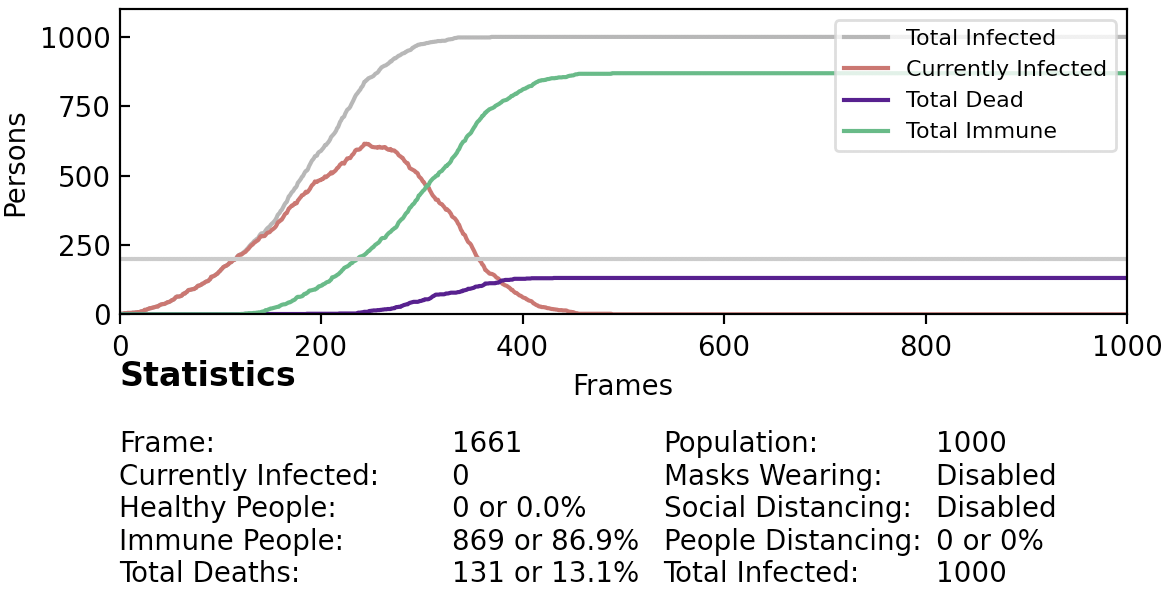
\includegraphics[width=10cm]{figures/population_density_1000.png}
    \caption{Virus Spread with Time for COVID-19 with Population Size = 1000}
    \label{population_density_1000}
\end{figure}

In Figure \ref{population_denisty_522}, we can see that the virus spreads slowly as people are distributed on the map in a more sparse manner. With a population size of only 522 distributed evenly on a map, the likelihood of a healthy person coming in contact with an infected person decreases. A small section of the people (30 people/5.7\%) end up not contracting the virus at all. 

\begin{figure}[H]
    \centering
    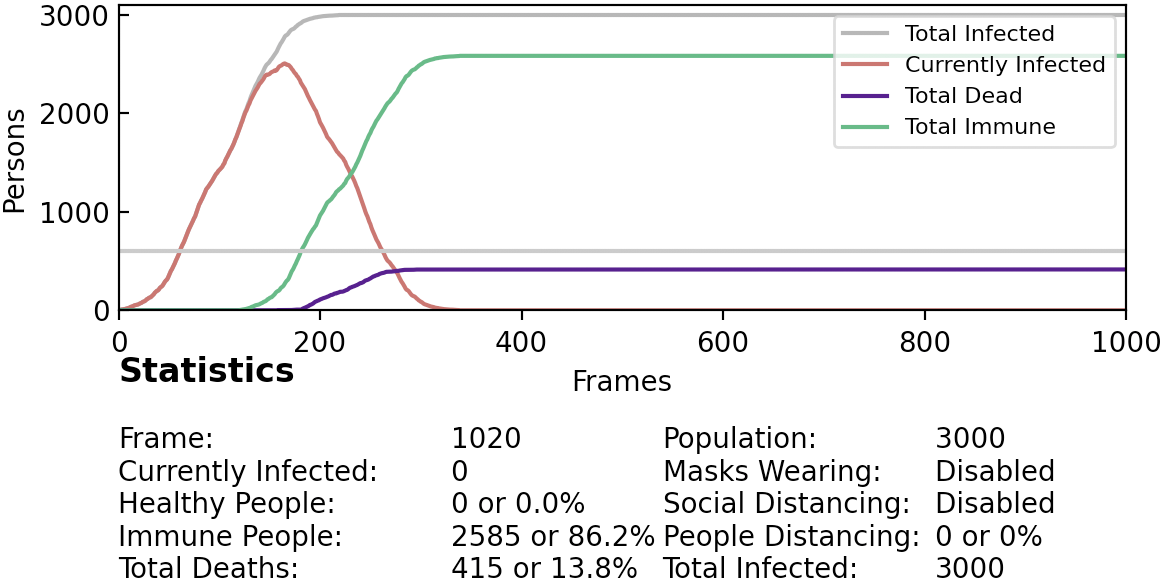
\includegraphics[width=10cm]{figures/population_density_3000.png}
    \caption{Virus Spread with Time for COVID-19 with Population Size = 3000}
    \label{population_density_3000}
\end{figure}

In Figure \ref{population_density_1000}, we can see that the virus spreads comparatively faster with the entire population contracting the disease at around 250$^\text{th}$ frame. 


In Figure \ref{population_density_3000}, we can see that the virus spreads the fastest with the entire population contracting the virus even before the 200$^\text{th}$ frame. This happens because the people are so densely populated in the same area that they are very likely to come in contact with a diseased person when there are no social distancing measures and high activity at all times. We observe that death rates between the population do not differ by all that much because as the population increases, the healthcare capacity scales up accordingly. This is consistent with our findings from our research \cite{covid_lowdeath}. 

\subsection{Mask Mandates} For mask mandates, we see that masks alone don't affect the number of cases drastically. This is because they do not protect an individual a 100\% from contracting the virus if they were to come within the infection range of an infected individual. Mask mandates do help flatten the curve so that the hospital capacities\cite{mask_wearing} are not overwhelmed We distribute 3 types of masks and have 4 cases configured for the population evenly:
\begin{enumerate}
    \item No Masks: Efficiency is 0\%
    \item Cloth Masks
    \item Surgical Masks
    \item N95 Masks
\end{enumerate}

We run 2 simulation experiments for COVID-19: no mask mandates, mask mandates starting at frame 70. Our results are reported in Figure \ref{no_mask_mandate}, \ref{mask_mandate}.

\begin{figure}[H]
    \centering
    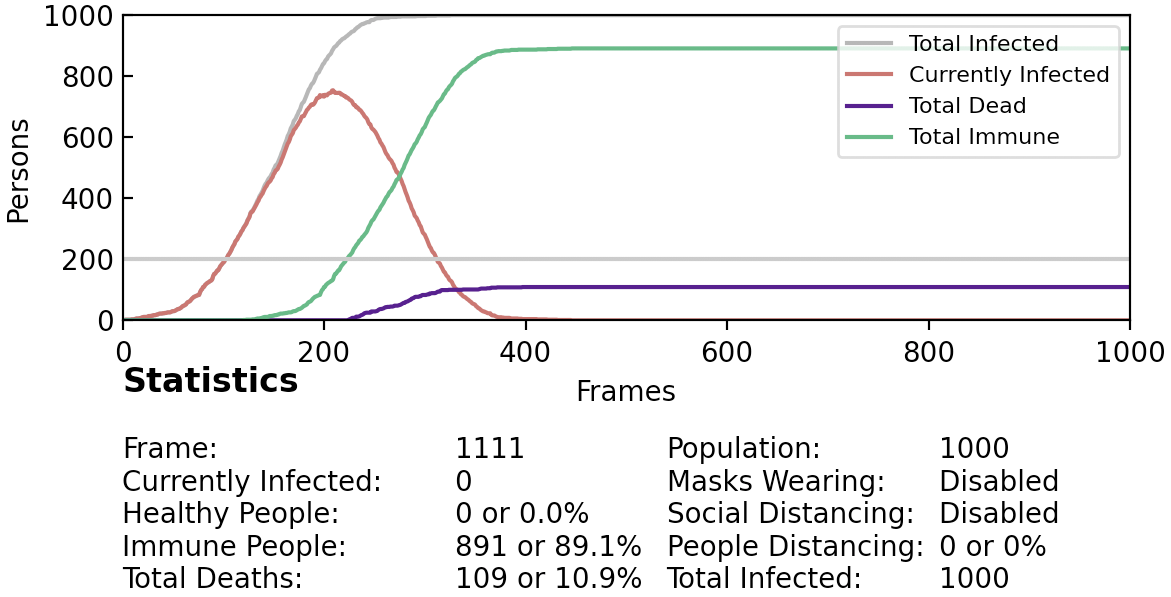
\includegraphics[width=10cm]{figures/no_mask_mandate.png}
    \caption{Virus Spread with Time for COVID-19 with No Mask Mandate}
    \label{no_mask_mandate}
\end{figure}

\begin{figure}[H]
    \centering
    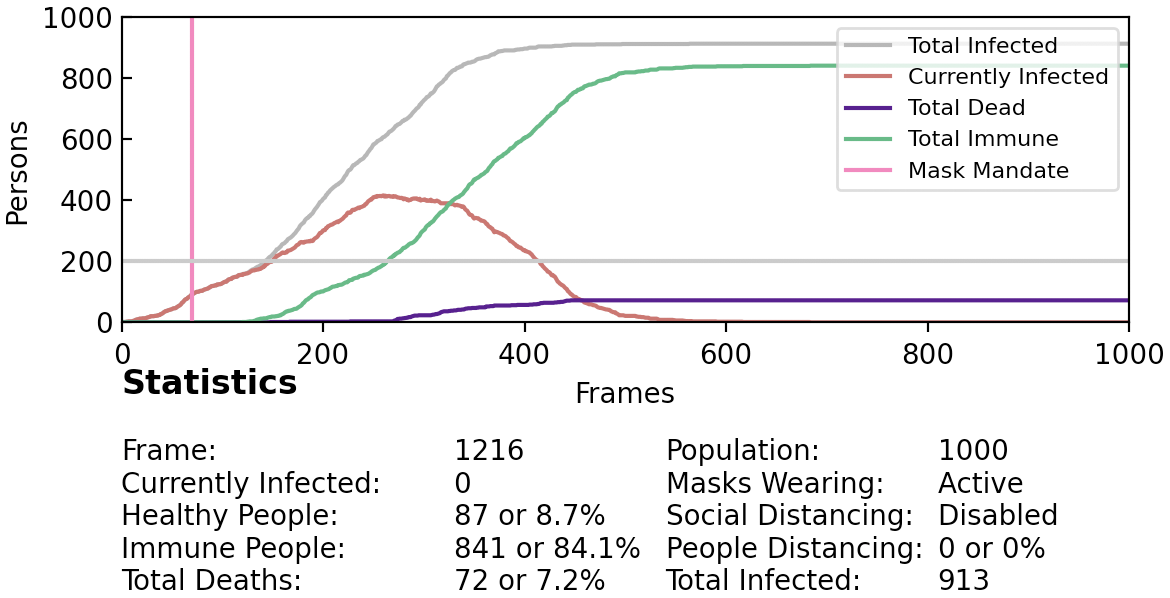
\includegraphics[width=10cm]{figures/mask_mandate.png}
    \caption{Virus Spread with Time for COVID-19 with Mask Mandate starting at Frame 70}
    \label{mask_mandate}
\end{figure}

As one can see, mask mandates don't change the total number of infections by much, however they do affect the death rates. By wearing masks, people flatten the curve of current infections, thereby, allowing hospitals to function more or less under their full capacity and having space for people to be hospitalized if they need it. In Figure \ref{mask_mandate}, the number of deaths are 72 (7.2\%) and the curve is more evenly spread out through time. At one point no more than 40\% of the population is infected. However, in Figure \ref{no_mask_mandate}, the curve for current infection is steeper, reaches the peak much earlier thereby overwhelming the hospital capacity and causing more deaths. In this scenario, 109 (10.9\%) people died which is much higher than for a mask mandate. 

\subsection{Healthcare Capacity}
The capacity of the healthcare facilities can affect the death rates drastically. If the virus grows faster and no control measures are taken, there are a large portion of people infected at the same time and the healthcare capacities are overwhelmed. This leads to a lot of people who may need medical intervention not get the help they need promptly or at all, thereby, causing their demise\cite{healthcare_capacity}. We found that hospital capacities are generally set as a percent of the total population. We run 3 simulation experiments: healthcare capacity is 20\% of the population, healthcare capacity is 50\% of the population, healthcare capacity is 80\% of the population. The results are reported in Figure \ref{hospital_capacity_20percent}, \ref{hospital_capacity_80percent}, \ref{hospital_capacity_80percent}.

 \begin{figure}[H]
    \centering
    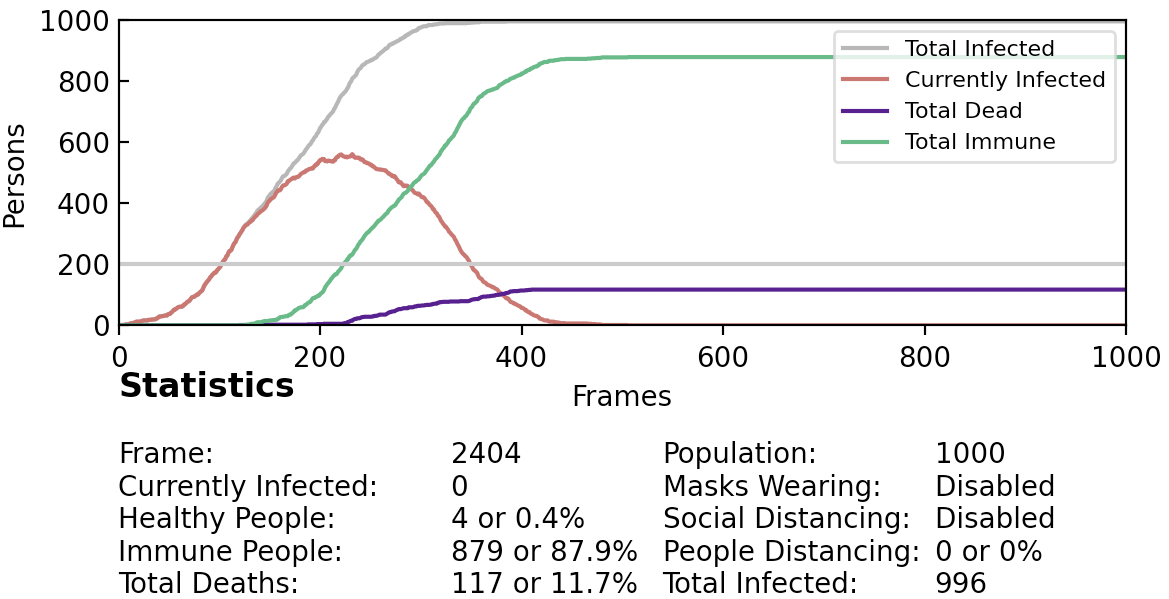
\includegraphics[width=10cm]{figures/hospital_capacity_20percent.png}
    \caption{Virus Spread with Time for COVID-19 with Hospital Capacity = 20\%}
    \label{hospital_capacity_20percent}
\end{figure}

\begin{figure}[H]
    \centering
    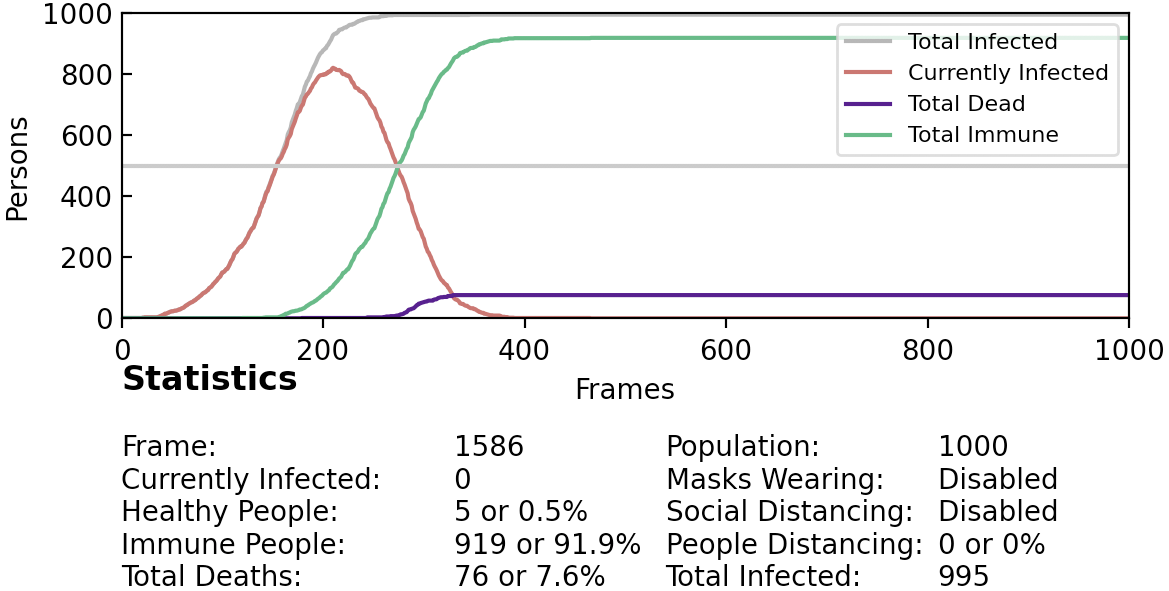
\includegraphics[width=10cm]{figures/hospital_capacity_50percent.png}
    \caption{Virus Spread with Time for COVID-19 with Hospital Capacity = 50\%}
    \label{hospital_capacity_50percent}
\end{figure}

\begin{figure}[H]
    \centering
    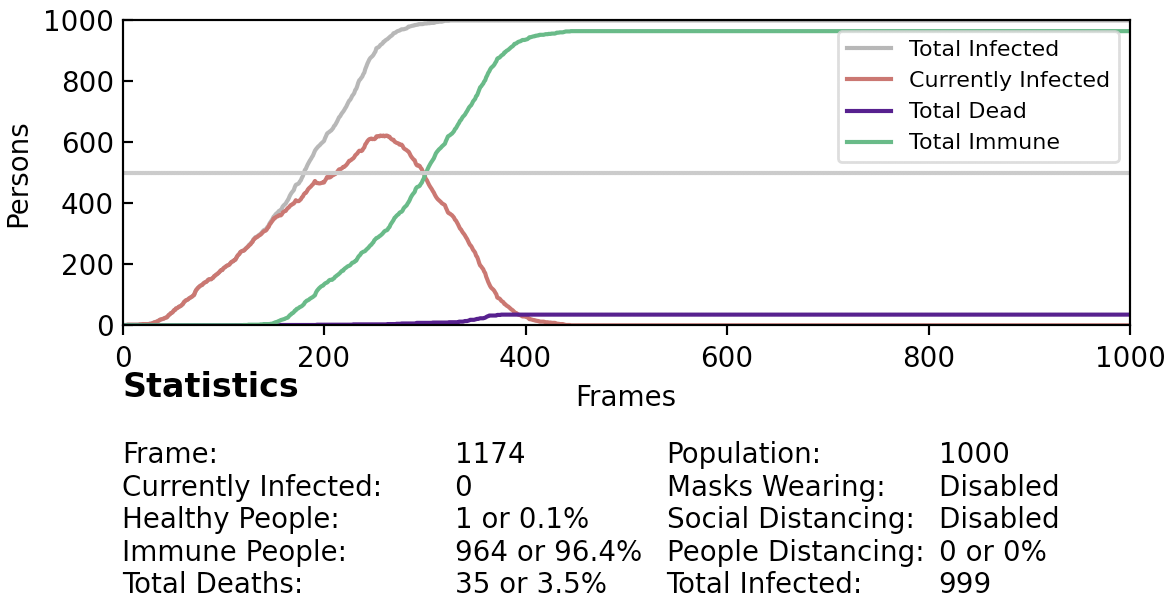
\includegraphics[width=10cm]{figures/hospital_capacity_80percent.png}
    \caption{Virus Spread with Time for COVID-19 with Hospital Capacity = 80\%}
    \label{hospital_capacity_80percent}
\end{figure}

In Figure \ref{hospital_capacity_20percent}, we can observe that with the hospital capacity being 20\% of the total population, the number of deaths were quite high i.e 117 people (11.7\%). This implies that a lot of people couldn't get the medical intervention that they needed. 

In Figure \ref{hospital_capacity_50percent}, with the hospital capacity being 50\% of the total population, the number of deaths decreased as the hospital could hold a larger amount of people. The number of deaths in this scenario were 76 people (7.6\%). 

In Figure \ref{hospital_capacity_80percent}, we have hospital capacity to be 80\% of the total population. This is an unlikely scenario because in a normal case, no one would expect more than even 40\% of the people to be hospitalized at the same time. However with the current COVID-19 pandemic, the surges in the infection affecting each individual differently, the hospitals are running at capacity and there are deaths which could've been prevented otherwise. In the Figure \ref{hospital_capacity_80percent}, one can see that only 35 people or 3.5\% of the population died as everyone got the medical intervention they needed because the hospital capacity was 80\% of the total population.

\subsection{Outbreak Control} 
After seeing our analysis above, one may ask: how can we control the outbreak as the vaccine is still not widely available to us? We here following the WHO guidelines\cite{who_guidelines} try to show that if social distancing and mask mandates are implemented early and followed by a large portion of the population, it is very much possible to be safe from the most devastating of outbreaks. For this experiment, we create a virus with a higher R value = 8, a lower K value (0.1) which means that there are more chances of superspreader events and 1 person can go on infect 8 people on an average. However, we make more than 50\% of the population practice social distancing and wear masks from an early stage. Our results are reported in Figure \ref{outbreak control}. 

\begin{figure}[H]
    \centering
    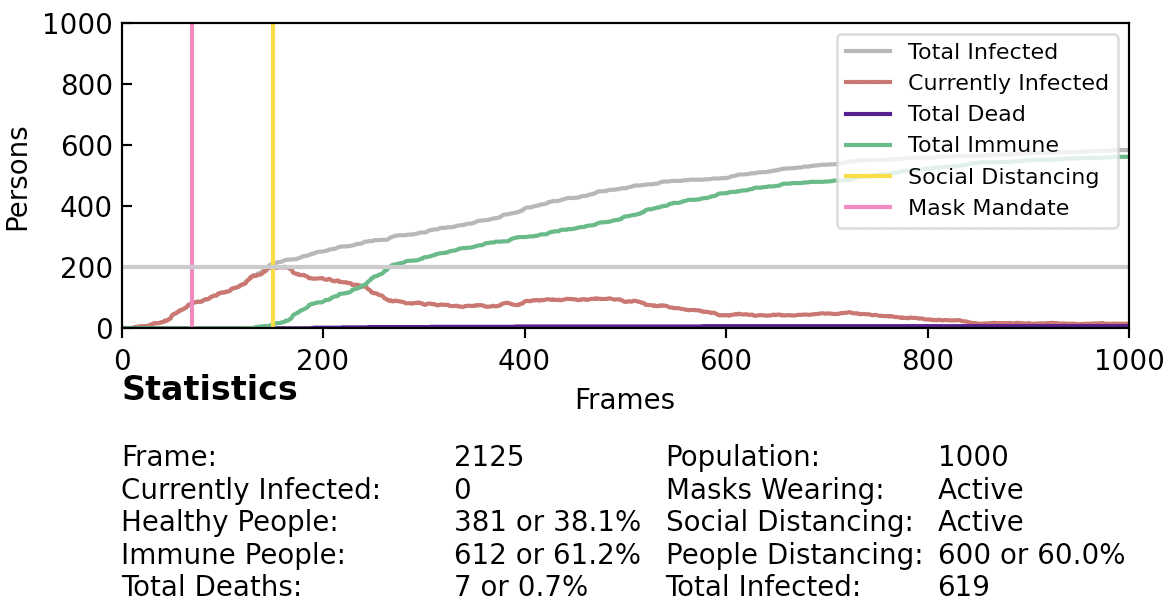
\includegraphics[width=10cm]{figures/outbreak_control.png}
    \caption{Virus Spread with Time for a Virus with R value = 8, K value = 0.1, 60\% of the Population Social Distancing Starting at Frame 150 and Mask Mandate starting at Frame 70}
    \label{outbreak control}
\end{figure}

The results in Figure \ref{outbreak control} is quite an optimistic but hopeful way of showing that even with a disease with a reproduction value (R value) = 8 and K value = 0.1, if more than 50\% of the people social distance and wear masks from an early stage of the outbreak, the number of cases can be controlled. One can also see that the current cases always remained under the hospital capacity and only 7 (0.7\%) people died. In our section for the R values, where no one was social distancing or wearing masks and the R value was 8 (please see Figure \ref{r_value_8}), the entire population got the infection before frame 200 and 152 people died (15.2\%). Here, 60\% of the population started social distancing from Frame 150, and started wearing masks at Frame 70. This immensely helped control the spread.

\subsection{Influenza vs COVID-19}
In our application, we have pre-loaded data for Influenza\cite{influ_ref}\cite{k_val} and COVID-19\cite{cov_ref}\cite{k_val}. These two viral diseases have very different characteristics. The tables are given in Table \ref{analysis-rk}, \ref{analysis-mortality}. 

\begin{table}[H]
\begin{tabular}{|l|l|l|}

\hline
          & R value & K value \\ \hline
COVID-19  & 3.00    & 0.1    \\ \hline
Influenza & 1.8     & 0.9    \\ \hline
\end{tabular}
    \caption{\label{analysis-rk}R and K values of COVID-19 and Influenza}
\end{table}

\begin{table}[H]
\begin{tabular}{|l|l|l|l|l|}

\hline
          & Mortality Rate: 0-19 & Mortality Rate: 20-49 & Mortality Rate: 50-69 & Mortality Rate: 70+ \\ \hline
COVID-19  & 0.003\%              & 0.02\%                & 0.5\%                 & 5.4\%               \\ \hline
Influenza & 0.02\%               & 0.05\%                & 0.06\%                & 0.86\%             \\ \hline
\end{tabular}
\caption{\label{analysis-mortality}Mortality Rate for 4 age groups for COVID-19 and Influenza}
\end{table}

We provide an analysis for both by running the simulation. Our results are reported in Figure \ref{covid-analysis}, \ref{influenza-analysis}. 

\begin{figure}[H]
    \centering
    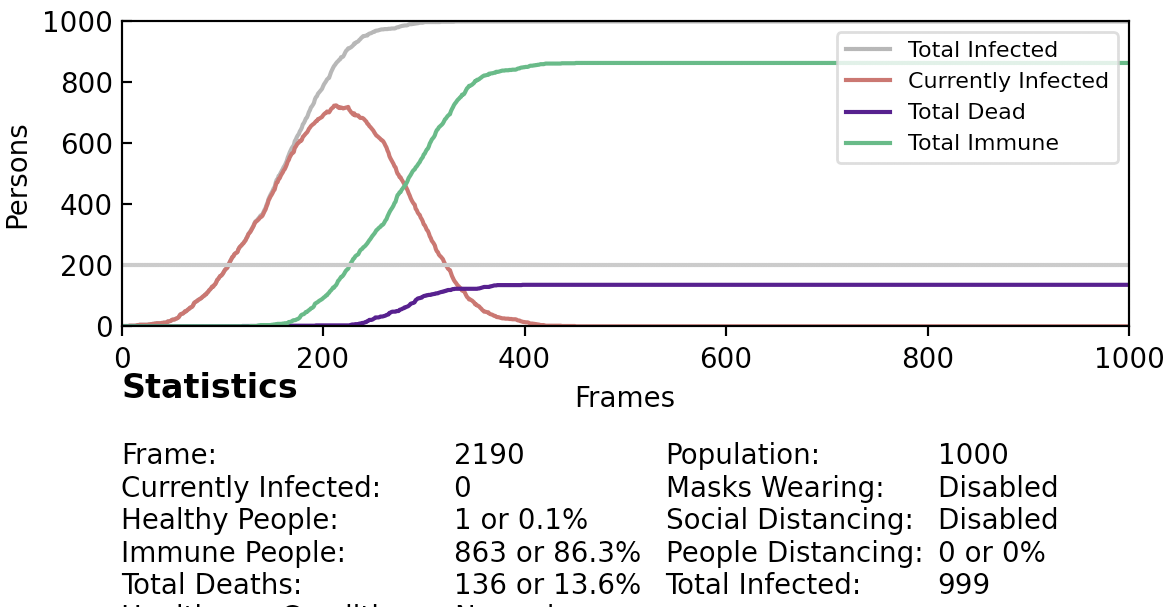
\includegraphics[width=10cm]{figures/covid-analysis.png}
    \caption{Virus Spread with Time with COVID-19 Virus}
    \label{covid-analysis}
\end{figure}

\begin{figure}[H]
    \centering
    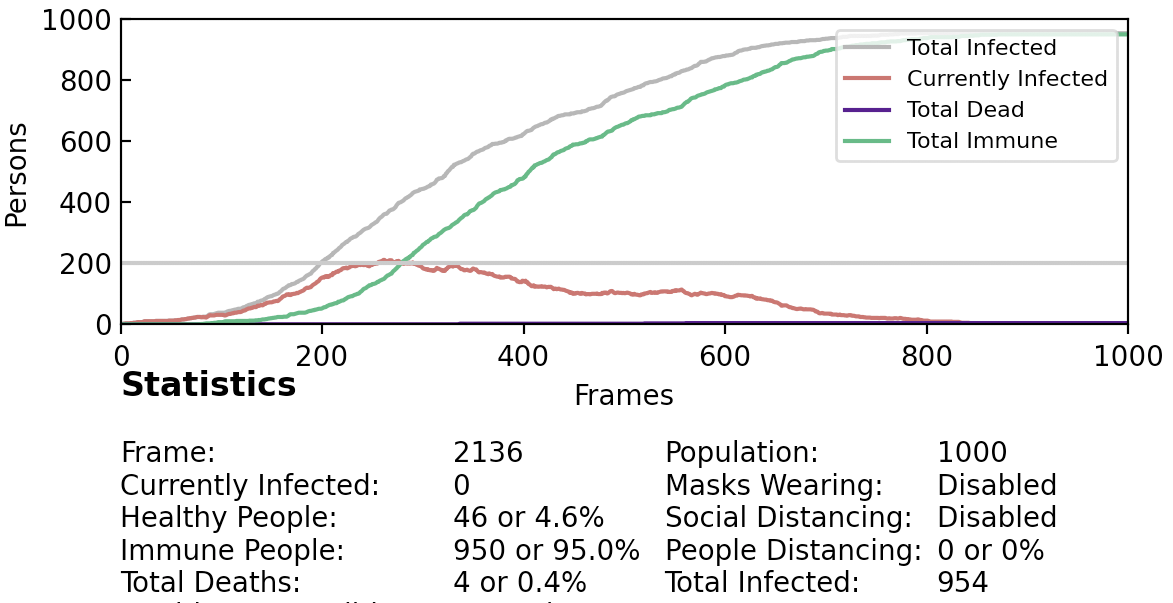
\includegraphics[width=10cm]{figures/influenza-analysis.png}
    \caption{Virus Spread with Time for Influenza Virus}
    \label{influenza-analysis}
\end{figure}

The results of our experiment simulations were as expected. As one can see, in COVID-19 virus (SARS-CoV-2), with a high R value and a low K value, there are more superspreader events and the virus grows rapidly. The entire population gets infected and the death toll 13.6\% of the total population or 136 people. In case of Influenza, with a R value of 1.8 and K value 0.9, the spread of the disease is much slower. Influenza having lower mortality rates brings the death toll to a comparatively very low number of only 0.4\% or 4 people.
\section{Conclusion} 
We developed an application capable of simulating a virus spread that took into account various factors such as the virus specific characteristics (R value, K value, recovery time, mortality rates, mask effectiveness) and population specific characteristics (population size, social distancing, mask mandates) to demonstrate an outbreak and its impact. From our analysis above, we found that the simulation model demonstrated results which were on par with our expectations, observations in real world, and our research. Some of the conclusions that can be made using our simulation models are:
\begin{enumerate}
    \item R and K value of a virus together can have a huge effect on how fast the virus spreads and its exponential growth. When R value is less than 1, that implies that the virus outbreak is contracting and will disappear by itself soon. K value affects the individual R value of a person; how many people the infected individual will spread the virus to. With a lower K value, the individual R value shows more variance and a person may thereby spread the virus to a lot of people (such as the case in superspreader events) or not spread the virus at all (being a deadend in terms of the spread). The most devastating impact of a virus occurs when a virus has a very high R value and a very low K value. We analyzed the individual impacts of R and K value in section 7.2 and 7.3. 
    \item Population density also plays a role in how fast a virus spreads. If a large amount of people are situated in small area, the virus will spread much faster as compared to a more sparsely populated region. This is consistent with our research \cite{density}. Of course, the impact of population density can be reduced by control measures such as social distancing and mask mandates which can also be seen in our analysis. Urban areas are in fact linked with lower infection rates for COVID-19 because they have higher healthcare capacity, more people social distancing, wearing masks and more awareness \cite{covid_urban}. Population density is also not linked with high death rates because the healthcare capacity is a function of the population size and hence, scales up accordingly allowing people to get the medical intervention that they may need\cite{covid_lowdeath}. The effects of high hospital capacity and control measures have been analyzed in section 7.7, 7.6 and 7.4 respectively.
    \item Flattening the curve can help reduce the death rates by allowing healthcare capacity to function normally. This is consistent with our research \cite{flatten_curve} that the longer the infection can be prevented, the more equipped an area is to deal with it. We analyze this in section 7.4, and 7.6. We demonstrate the effect of healthcare capacity in section 7.7
    \item With appropriate control measures in place, even virus with an R value as high as 8 with a potential to have devastating consequences can be controlled early. This requires social distancing and mask wearing to be implemented as early as possible. We analyzed outbreak control in section 7.8 and analyzed the individual effects of social distancing and mask wearing in section 7.4 and 7.6 respectively. It is imperative that a larger portion of the population follow these control measures in order to prevent higher surges in infections. It is the responsibility of the area officials to put appropriate control measures for the public as early as possible.

    
\end{enumerate}

\pagebreak
\listoffigures
\listoftables
\bibliographystyle{unsrt}
\bibliography{references.bib}
\end{document}
